% Modelo de Dissertacoes do Mestrado em Informatica da PUC
\documentclass[a4paper,brazil,ruledheader,normaltoc,capchap]{abnt}

%\usepackage{fancyhdr}

% Usar a fonte Times New Roman
\usepackage{pslatex}

% Pacotes de codificacao das fontes para portugues
\usepackage[T1]{fontenc}
\usepackage[ansinew]{inputenc}

%\usepackage{units}		% Utilize da seguinte forma  \unit[78,6]{mA}

\usepackage[printonlyused]{acronym}

% Merge em duas celulas (linhas diferentes)
\usepackage{multirow}

% Pacote para citacao e referencias seguindo ABNT no sistema (AUTOR, Data)
\usepackage[alf]{abntcite}

% Pacote para divisao silabica do portugues
\usepackage[brazil]{babel}

% Pacote de adequacao do formato ABNT para normas da PUCMinas
\usepackage{abnt-PPGInf-PUCMG}

% Pacotes utilitarios
\usepackage[pdftex]{graphicx}
\usepackage{epstopdf}

\usepackage[all]{xy}
\usepackage[tight]{subfigure}	% Permite a criacao de subfiguras
%\usepackage{url,amsmath}		% Permite melhorias na codificacao de formulas
%\usepackage{amsthm}			% Permite melhorias na escrita de teoremas
%\usepackage{amssymb}			% Permite utlizacao de simbolos matematicos avancados

\usepackage[english, linesnumbered, ruled, vlined]{algorithm2e}
\usepackage{algorithmic} %algorithm
\usepackage{listings}

% Alterar o espacamento da margem no algoritmo
\setlength{\algomargin}{1em}
\usepackage{setspace}
\usepackage{acronym}

% Pacote para rotacao de tabelas/figuras
\usepackage{rotating}

% Pacotes para criacao de cronograma/tabela colorida
%\usepackage{auto-pst-pdf}
\usepackage{epstopdf}
\usepackage{graphics}
%\usepackage{pstricks}
\usepackage{color}
\usepackage{array}
\usepackage{longtable}
\usepackage{colortbl}

%Suporte a visualiza��o landscape
\usepackage{lscape}

% Para inserir captions
\usepackage[size=normalsize,bf,center]{caption}

\setlength{\LTcapwidth}{\textwidth}

\makeatletter
\renewcommand\chapter{\par%
  %\setcounter{page}{2}
  \global\@topnum\z@
  \@afterindentfalse
  \secdef\@chapter\@schapter}
\makeatother
%\renewcommand{\ALG@name}{Algoritmo}
%\renewcommand{\listalgorithmname}{Lista de Algoritmos}


% Codigo
\lstset{numbers=left,
stepnumber=1,
firstnumber=1,
numberstyle=\tiny,
extendedchars=true,
breaklines=true,
frame=htb,
basicstyle=\footnotesize,
stringstyle=\ttfamily,
showstringspaces=false
}
%\renewcommand{\lstlistingname}{C+�digo}
%\renewcommand{\lstlistlistingname}{Lista de C+�digos}
\citeoption{abnt-etal-cite=3, abnt-and-type=e}

%%%%%%%%%%%%%%%%%%%%%%%%%%%% PR�-TEXTUAIS %%%%%%%%%%%%%%%%%%%%%%%%%%
\begin{document}

% Alterar o t�tulo das refer�ncias para somente 'Refer�ncias'
\renewcommand{\bibname}{Refer�ncias}

\autor{Dayana Thalita Santos Viana}

% Coloque o t�tulo em caixa alta. � o padr�o da PUC.
% V� no arquivo abnt-PPGInf-PUCMG.sty e procure por esse t�tulo (linha 575). Altere para o seu t�tulo, sem ser em caixa alta. Isso ser� utilizado na folha de aprova��o.
\titulo{PROCESSO DE KDD APLICADO AOS MICRODADOS DO CENSO DA EDUCA��O SUPERIOR DO INEP}

\orientador[Orientador:]{Hugo Bastos de Paula}

% Se n�o tiver, co-orientador, comente a pr�xima linha.
%\coorientador[Co-orientador:]{Professor}

% Texto
\comentario{Monografia apresentada ao Curso de Sistemas de Informa��o da Pontif�cia Universidade Cat�lica de Minas Gerais, como requisito parcial para obten��o do t�tulo de Bacharel Sistemas de Informa��o.}

% Institui��o
\instituicao{PONTIF�CIA UNIVERSIDADE CAT�LICA DE MINAS GERAIS \par Bacharelado em Sistemas de Informa��o}

% Local
\local{Belo Horizonte}

% Data
\data{2012}

% Gera a capa
\capa

% Gera a folha de rosto
\folhaderosto

% Ficha catalogr�fica
% Deve ser impressa atr�s da folha de rosto!!!!
%% Ficha catalogr�fica
\newpage

% Espa�amento do topo da p�gina at� a ficha catalogr�fica
\vspace*{11cm}

% Utilizar espa�amento de 1.5
\onehalfspacing

% Tabela com a ficha catalogr�fica
\begin{table}[h]

	% Tamanho da letra
	\footnotesize

	% Tabela centralizada
	\centering

	%T�tulo
	\caption*{\small FICHA CATALOGR�FICA}

	% Conte�do
	% Altere somente os textos necess�rios. N�o tire os '~', pois eles for�am o espa�amento na esquerda.
	% Para adicionar novas linhas, use o texto a seguir para cada nova linha:
	% & & ~~~ Texto \\
	\begin{tabular}{c|p{1,6cm}p{10,5cm}|}
	\multicolumn{3}{l}{~~~ Elaborada pela Biblioteca da Pontif�cia Universidade Cat�lica de Minas Gerais} \\ \cline{2-3}
	& & \\
	& & Viana, Dayana Thalita Santos \\
	& R484r  & ~~~ Processo de KDD aplicado aos microdados do censo da educa��o superior do Inep ~~ / Dayana Thalita Santos Viana. -- Belo Horizonte, \\
	& & 2012.\\
	& & ~~~ 103f. : il.\\
	& &\\
	& & ~~~ Orientador: Hugo Bastos de Paula\\
	% Comente a pr�xima linha se n�o houver co-orientador
	%& & ~~~ Co-orientador: Luis Enrique Z�rate\\ 
	& & ~~~ Monografia (Gradua��o) -- Pontif�cia Universidade Cat�lica de\\
	& & ~~~ Minas Gerais. Programa de Gradua��o em Sistemas de Informa��o\\
	& & ~~~ - Instituto de Inform�tica.\\
	& & ~~~ Bibliografia.\\
	& & \\
	& & ~~~ 1. Microdados do Censo da Educa��o Superior. 2. Minera��o de \\
	& & ~~~ Dados. 3. SQL Server 2012. I. Pontif�cia Universidade Cat�lica\\
	& & ~~~ de Minas Gerais. II. Artigos e Sites da Intenet. III. Programa\\
	& & ~~~ Microsoft Student to Business (S2B) IV. T�tulo. \\
	& & \\
	% Altere apenas do CDU: ####
	& & ~~~~~~~~~~~~~~~~~~~~~~~~~~~~~~~~~~~~~~~~~~~~~~~~~~~~~~~~~~~~~~~~~~~~~~~~~~~CDU: 681.3.01:621.39 \\ \cline{2-3}
	% Altere apenas o nome do bibliotec�rio e o CRB6/1084. N�o tire os '~', pois eles for�am o espa�amento na esquerda.
	\multicolumn{3}{l}{~~~ Bibliotec�rio: Fernando A. Dias -- CRB6/1084} \\
	\end{tabular}
\end{table}

% Altera a fonte para o tamanho normal
\normalsize


% Folha de aprova��o
% Termo de Aprova��o

% Texto da aprova��o
\textoaprovacao{Monografia apresentada ao Curso de Sistemas de Informa��o da Pontif�cia Universidade Cat�lica de Minas Gerais, como requisito parcial para obten��o do t�tulo de Bacharel Sistemas de Informa��o.}

% Primeira assinatura
\primeiroassina{Professor 1 (Orientador) -- PUC Minas}

% Segunda assinatura
%\segundoassina{Professor 2 (Co-orientador) -- PUC Minas}

% Terceira assinatura
\terceiroassina{Professor 2 -- PUC Minas}

% Quarta assinatura
\quartoassina{Professor 3 -- Universidade}

% Data da defesa
\localdia{Belo Horizonte, 26 de Novembro de 2012.}

% Gera o termo de aprova��o
\termodeaprovacao

% OU, SE FOR UM ARQUIVO PDF, J� COM AS ASSINATURAS, BASTA INCLUIR O ARQUIVO COMO FIGURA.
%\begin{figure}[h!]
%	\vspace*{-3.3cm}
%	\hspace*{-3cm}
%    % Suponha o nome do arquivo em pre-texto/folha-aprovacao/folhaaprovacao.pdf
%	\includegraphics{pre-texto/folha-aprovacao/folhaaprovacao} 
%	\newpage
%\end{figure}


% Dedicat�ria
% Dedicat�ria
\newpage

% Espa�amento do topo da p�gina at� o texto da dedicat�ria
\vspace*{17cm}

% Texto da dedicat�ria alinhado a direita
\begin{flushright}
\textit{A toda minha fam�lia e principalmente ao meu pai, \\por ter me dado todo carinho e a melhor educa��o poss�vel, \\e por ser um grande exemplo de boa pessoa.}
\end{flushright}


% Agradecimentos
% Agradecimentos
\chapter*{Agradecimentos}

Ao Prof. Hugo Bastos, pela orienta��o neste trabalho de conclus�o de curso.

Aos demais professores, que compartilharam seus conhecimentos e experi�ncias.

Aos colegas do curso de Sistemas de Informa��o da PUC Minas.

E a minha fam�lia pelo apoio e compreens�o durante todo esse per�odo.


% Ep�grafe
% Ep�grafe
\newpage

% Espa�amento entre topo da p�gina e texto da ep�grafe
\vspace*{8cm}
% Espa�amento na esqueda
\hspace{3cm}\begin{minipage}{.51\textwidth}

% Texto da ep�grafe
\textit{``Suba o primeiro degrau com f�. \\N�o � necess�rio que voc� veja toda a escada. \\Apenas d� o primeiro passo.'' }

% Nome do autor
\begin{flushright}\itshape Martin Luther King\upshape\end{flushright}

\end{minipage}


% Resumo
% Resumo
\begin{resumo}

% Texto do resumo, em portugu�s: sem par�grafo, alinhado � esquerda
\noindent 

O \ac{KDD} � um processo composto de v�rias etapas para compreens�o de padr�es nos dados. Dada a divulga��o p�blica dos dados do Censo da Educa��o Superior realizada anualmente pelo \ac{Inep} temos uma base de dados para desenvolver o processo. Foi utilizada Minera��o de Dados, com o aux�lio de ferramentas como o SQL Server e Excel para descoberta de conhecimento nessa base de dados. Visto que um dos maiores desafios que o ensino superior enfrenta hoje � prever as decis�es dos alunos, a utiliza��o desse processo e ferramentas pode ajudar a tomada de decis�es da Universidade PUC Minas. Os resultados trouxeram informa��es e previs�es sobre ingressos e evas�es; an�lises sobre a quantidade de candidatos vaga; a import�ncia do curso de Sistemas de Informa��o dentro e fora da PUC Minas; influenciadores da taxa de ocupa��o, principais cursos que aparecem juntos com grande ocupa��o e recomenda��es.

% Espa�amento para as palavras-chave
\vspace*{.75cm}

% Palavras-chave: sem par�grafo, alinhado � esquerda
\noindent Palavras-chave: Processo KDD. SQL Server. Excel. ETL. Minera��o de Dados.  \\
% Segunda linha de palavras-chave, com espa�amento.
\indent\hspace{2cm}Censo da Educa��o Superior.

\end{resumo}


% Abstract
%% Abstract
\begin{abstract}

% Texto do resumo, em ingl�s: sem par�grafo, alinhado � esquerda
\noindent \ac{KDD} is one process that consists of several steps to understanding patterns in data. Given the public disclosure of data from the Census of Higher Education conducted annually by Inep we have a great database to develop the process. Data Mining was used, with the aid of tools such as SQL Server and Excel for knowledge discovery in this database. Since one of the biggest challenges that higher education faces today is predicting the decisions of students, the use of this process and tools can help decision making at the University PUC Minas.

% Espa�amento para as palavras-chave
\vspace*{.75cm}

% Palavras-chave: sem par�grafo, alinhado � esquerda
\noindent Keywords: KDD Process. SQL Server. Excel. ETL. Data Mining. \\
% Segunda linha de palavras-chave, com espa�amento.
\indent\hspace{1.4cm}Census of Higher Education.

\end{abstract}


% Lista de figuras
\listoffigures

% Lista de tabelas
\listoftables

% Lista de siglas
\newpage
% Lista de Abreviaturas e Siglas
\chapter*{Lista de Abreviaturas e Siglas}

% Mantenha sempre em ordem alfab�tica.

\begin{acronym}
\acro{BI}{\textit{Business Inteligence}}
\acro{DCBD}{Descoberta de Conhecimento em Banco de Dados}
\acro{DW}{\textit{Data Warehouse}}
\acro{ETL}{\textit{Extract Transform Load}}
\acro{GTI}{Ger�ncia de Tecnologia de Informa��o}
\acro{IES}{Institui��es de Ensino Superior}
\acro{Inep}{Instituto Nacional de Estudos e Pesquisas Educacionais An�sio Teixeira}
\acro{KDD}{\textit{Knowledge Discovery in Databases}}
\acro{OLAP}{\textit{On-Line Analytical Processing}}
\acro{PUC Minas}{Pontif�cia Universidade Cat�lica de Minas Gerais}
\acro{SGBD}{Sistema Gerenciador de Banco de Dados}
\acro{S2B}{\textit{Students to Business}}
\end{acronym}


% Sum�rio
\tableofcontents

%%%%%%%%%%%%%%%%%%%%%%%%%%%%% TEXTUAIS %%%%%%%%%%%%%%%%%%%%%%%%%%%
\clearpage

% Altere o numero da pagina para o correto. Conte todas as paginas, menos a capa, inclusive a ficha catalografica ate a pagina do primeiro capitulo.

\newpage
\pagenumbering{arabic}
\pagestyle{myheadings}
\setcounter{secnumdepth}{5}


% Cap�tulos
\sumario
\capitulo{INTRODUÇÃO}

\secao{Contextualização}

Instituições de ensino universitarias se deparam todo início de semestre letivo com o problema de alocação de salas, este problema pode ser definido como \textit{Classroom Assignment} que é uma instancia do \textit{course timetabling}, problemas desta instancia são prolemas de otimização combinatoria. Problemas de otimização combinatoria tem a complexidade NP-difícil, para a resolução de problemas desta complexidade em um tempo razoavel são propostas algumas tecnicas denominadas meta-heuristicas. Esta técnicas amenizam a dificildade da resolução destes problemas para encontrar uma solução em um tempo habil, uma vez que, a resolução destes problemas de forma manual é de grande dificuldade em alguns casos pode demandar semanas de trabalho da pessoa responsável.\par


Em suma o trabalho consiste na distruições das disciplinas pertecentes aos cursos de graduação e pós-graduação apresentados po alguns  colegiados da Universidade Federal de Minas Gerais (UFMG) , em salas disponibilizadas pelo predio da Faculdade de Filosofia e Ciências Humandas (FAFICH). Para a distribuição destas disciplinas nas salas, foi criado um sistema que utiliza conceitos de algorítimo genético para resolver o problema PAS. Esta demanda de alocação acontece todo início de semestre e é executada assim que todos os colegiados tenham enviados suas solicitações necessidas para aquele semestre.\par

Uma vez que os termos da biologia utilizados foram lincados com o problema, o sistema gera uma alocação com grandes chances de atender as necessidades da instituição. \par

\secao{Objetivos}

O tratamento do problema de alocação de salas em instituições de ensino carece de bons trabalhos na literatura. Apesar de se encontrar ferramentas disponíveis, poucas tratam de maneira eficiente as restrições reais existentes nas instiruições. Com este trabalho objetiva-se:

\subsecao{Objetivos Gerais}

O objetivo deste trabalho é utilizar os conceitos de algoritimo genético para a resolução dos problemas denominados PAS através do desenvolvimento de um sistema que atenda todas as necesssidades da instiruição e facilite o gerenciamento das informações da instituição como salas, disciplinas e demais informações.

\subsecao{Objetivos Específicos}

	- Desenvolvimento do sistema.\par

	- Implementação de um algoritmo que proporcione uma solução de qualidade.

	- Otimizar o tempo do gestor.\par

	- Eficiência na geração dos relatórios.\par

\secao{Justificativa}

A solução de problemas de PAS através de meta-heurísticas se trata de uma área ainda não consolidada, por mais que existam trabalhos relacionados ao tema espera-se que as conclusões realizadas neste trabalho agreguem valor algum falor para os trabalhos futuros.

\secao{Organização do Trabalho}

Este trabalho está definido da seguinte forma, foi dividido em seis capítulos, sendo este capítulo 1 e mais cinco outros.\par

O capítulo 2 apresenta o referencial teórico do trabalho, descrevendo os conceitos utilizados para o desenvolvimento do projeto proposto: conceitos de TimeTable e Heurísticas.\par

No capítulo 3 é apresentada a metodologia do sistema e as tecnologias adotadas para desenvolvimento da solução.\par

No capítulo 4 iremos descrever e citar detalhadamente as características e propostas de desenvolvimento do sistema desenvolvido, proposto para este trabalho.\par

A conclusão deste trabalho e considerações finais são mostrados nos capítulos 5 e 6.\par

\cite{Date2000}

% Nome do capitulo
\chapter{KDD}
% Label para referenciar
\label{cap:kdd}
% Diminuir espacamento entre titulo e texto
\vspace{-1.9cm}

% Texto do capitulo
Diversas nota��es para encontrar padr�es �teis nos dados j� foram usadas. Entre elas, o termo \textit{data mining} foi o mais comum. A express�o \textit{Knowledge discovery in database} (KDD) apenas come�ou a ser usada em um workshop em 1989 para enfatizar que o conhecimento (\textit{knowledge}) era o produto final da procura. \ac{KDD} representa todo processo de descoberta de conhecimento. Inclui como os dados ser�o armazenados, acessados, como os algoritmos ser�o aplicados, como os resultados ser�o interpretados e visualizados. Por�m a �nfase maior se d� ao entendimento dos padr�es que podem ser interpretados como conhecimento �til.  J� \textit{data mining} � a aplica��o de algoritmos aos dados para obten��o de regras. � a modelagem de algoritmos para uma grande quantidade de dados inconsistentes \cite{Fayyad1996}.

KDD � um processo n�o trivial de identifica��o v�lida, �tima, �til e de f�cil compreens�o dos padr�es nos dados. O termo processo implica que o KDD possui diversos passos como a prepara��o dos dados, busca de padr�es, avalia��o do conhecimento e refinamento em m�ltiplas itera��es em que podem conter revis�es a cada dois passos. N�o trivial significa que s�o necess�rias pesquisas em cima dos dados e n�o somente computa��o com valores predefinidos. �til induz dizer que trar� algum benef�cio ao usu�rio ou suas tarefas \cite{Fayyad1996}.

O KDD � um processo interativo e iterativo que envolve diversos passos envolvendo decis�es feitas pelo usu�rio. Primeiramente � feito um estudo do dom�nio da aplica��o identificando qual � o conhecimento relevante para se atingir o objetivo. Em seguida, os dados coletados s�o selecionados focando em um subconjunto em que a descoberta ser� focada. O terceiro passo trabalha com a limpeza e processamento dos dados. Nesse passo as informa��es erradas, inconsistentes e at� mesmo inexistentes s�o manipuladas. A redu��o e proje��o fazem parte do quarto passo, onde caracter�sticas que representam os dados de acordo com o objetivo s�o encontradas. O quinto passo consiste em casar os objetivos do processo de KDD a um processo de \textit{data mining}, como por exemplo, clusteriza��o, classifica��o, sumariza��o, regress�o e etc. O sexto passo consiste na an�lise, modelagem e hip�tese, onde s�o analisados os modelos e par�metros mais apropriados. Os resultados s�o interpretados possibilitando o retorno aos passos 1 a 6 para mais itera��es. Finalmente o s�timo passo consiste na busca por padr�es de interesse representado em tabelas ou outros tipos de exibi��es. Como resultado podemos ter uma a��o usando o conhecimento adquirido, ou simplesmente produ��o de uma documenta��o a ser mostrada �s partes interessadas. Mesmo considerando todos os passos muito importantes, a parte mais trabalhosa do KDD est� no passo 5, o \textit{data mining} \cite{Fayyad1996}.

% Figura
\begin{figure}[ht]
	\caption{\textbf{Processo KDD} (Tradu��o por Dayana Viana)}
	\centering
	% Alterar espa�amentos antes e depois do caption
	\setlength{\abovecaptionskip}{0pt}
	\setlength{\belowcaptionskip}{0pt}
	% Arquivo da figura
	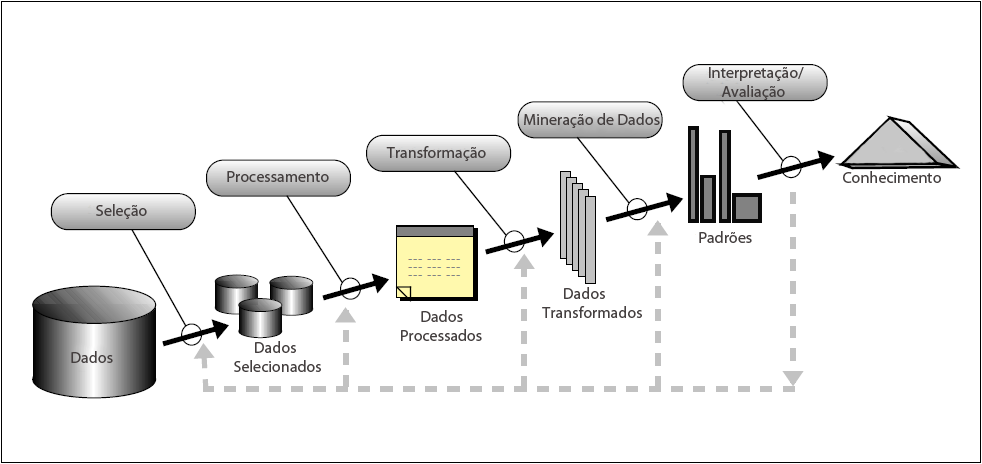
\includegraphics[width=.9\textwidth]{imagem/figura1.png}
	% Caption centralizada
	\captionsetup{justification=centering}
	% Caption e fonte
	\\
	\small{Fonte: \cite{Fayyad1996}}
	\label{img:kdd}
\end{figure}
% Nome do capitulo
\chapter{Minera��o de Dados}
% Label para referenciar
\label{cap:mineracao}
% Diminuir espacamento entre titulo e texto
\vspace{-1.9cm}

% Texto do capitulo
Assim como na minera��o geol�gica (carv�o, ouro, etc), n�o h� a garantia da obten��o de resultados significativos pela simples aplica��o das ferramentas ao terreno. Uma enorme prepara��o � necess�ria. Primeiramente, os dados devem estar preparados. A partir da� � poss�vel fazer a modelagem a fim de transform�-los em informa��es capazes de serem interpretadas pelos seres humanos. Modelar significa encontrar rela��es, fazer previs�es dos dados para descrever a situa��o atual. Os fundamentos dos m�todos utilizados para minera��o s�o f�ceis de entender, por�m sua implementa��o j� requer poderosos e sofisticados algoritmos para fazer com que esses m�todos funcionem na pr�tica \cite{Pyle1999}.

Atrav�s da observa��o da Figura \ref{img:mineracao} � poss�vel percebermos grupos formados pelos pontos. As ferramentas de modelagem tem como tarefa separar e agrupar os dados, nesse caso representado como pontos, de maneira com que tenham significado. Cada algoritmo realiza essa tarefa utilizando abordagens ligeiramente diferentes \cite{Pyle1999}. 

% Figura
\begin{figure}[ht]
	\caption{\textbf{Minera��o de Dados}}
	\centering
	% Alterar espa�amentos antes e depois do caption
	\setlength{\abovecaptionskip}{0pt}
	\setlength{\belowcaptionskip}{0pt}
	% Arquivo da figura
	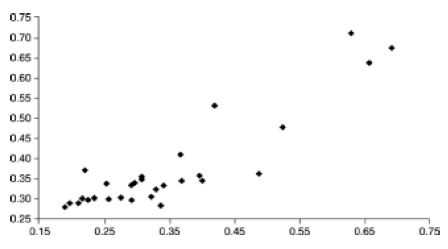
\includegraphics[width=.7\textwidth]{imagem/figura2.png}
	% Caption centralizada
	\captionsetup{justification=centering}
	% Caption e fonte
	\\
	\small{Fonte: \cite{Pyle1999}.}
	\label{img:mineracao}
\end{figure}

A minera��o de dados, componente do processo KDD, envolve aplica��o iterativa e repetida de um m�todo particular.  Ajustando os modelos obt�m-se padr�es a partir dos dados observados. A maioria dos m�todos de \textit{data mining} � baseada em experi�ncias e t�cnicas de testes das m�quinas de aprendizado, reconhecimento de padr�es e estat�sticas. Algumas t�cnicas de minera��o de dados s�o: �rvores de decis�o, clusteriza��o, vizinho mais pr�ximo e regress�o \cite{Fayyad1996}.

�rvores de Decis�o: Algoritmo baseado no processo de parti��o. As parti��es visando a separa��o dos pontos s�o feitas atrav�s de pontos de decis�es at� algum crit�rio de parada ou at� n�o ser mais poss�vel realizar separa��es (Figura \ref{img:arvore}) \cite{Pyle1999}.

% Figura
\begin{figure}[ht]
	\caption{\textbf{�rvores de Decis�o}}
	\centering
	% Alterar espa�amentos antes e depois do caption
	\setlength{\abovecaptionskip}{0pt}
	\setlength{\belowcaptionskip}{0pt}
	% Arquivo da figura
	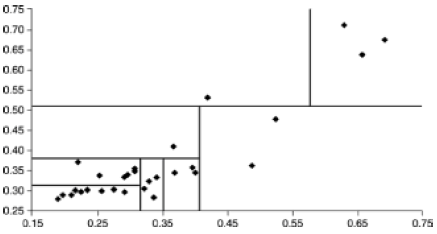
\includegraphics[width=.7\textwidth]{imagem/figura3.png}
	% Caption centralizada
	\captionsetup{justification=centering}
	% Caption e fonte
	\\
	\small{Fonte: \cite{Pyle1999}.}
	\label{img:arvore}
\end{figure}

Clusteriza��o: Tamb�m particionam os espa�os, por�m agrupando pontos que compartilham as mesmas caracter�sticas. Existem diferentes m�todos de clusteriza��o, mas todos produzem esse tipo de arranjo. Uma grande diferen�a desse m�todo � que ele n�o separa os grupos linearmente, o que facilita o encontro de similaridades (Figura \ref{img:cluster}) \cite{Pyle1999}.\\

% Figura
\begin{figure}[ht]
	\caption{\textbf{Clusteriza��o}}
	\centering
	% Alterar espa�amentos antes e depois do caption
	\setlength{\abovecaptionskip}{0pt}
	\setlength{\belowcaptionskip}{0pt}
	% Arquivo da figura
	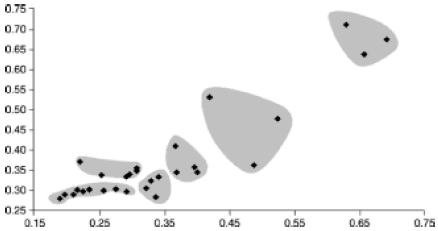
\includegraphics[width=.7\textwidth]{imagem/figura4.png}
	% Caption centralizada
	\captionsetup{justification=centering}
	% Caption e fonte
	\\
	\small{Fonte: \cite{Pyle1999}.}
	\label{img:cluster}
\end{figure}

Vizinho mais pr�ximo: Um tipo de classifica��o utilizado para descrever intera��es. Esse m�todo seleciona um n�mero espec�fico de vizinhos e para cada ponto calcula a vizinhan�a. A Figura \ref{img:visinho} ilustra como os vizinhos podem ser selecionados. Para cada ponto foi calculado os quatro vizinhos mais pr�ximos \cite{Pyle1999}.\\

% Figura
\begin{figure}[ht]
	\caption{\textbf{Vizinho mais pr�ximo}}
	\centering
	% Alterar espa�amentos antes e depois do caption
	\setlength{\abovecaptionskip}{0pt}
	\setlength{\belowcaptionskip}{0pt}
	% Arquivo da figura
	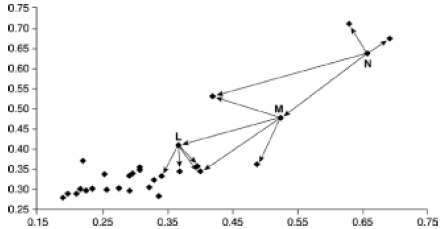
\includegraphics[width=.7\textwidth]{imagem/figura5.png}
	% Caption centralizada
	\captionsetup{justification=centering}
	% Caption e fonte
	\\
	\small{Fonte: \cite{Pyle1999}.}
	\label{img:visinho}
\end{figure}

Redes Neurais e Regress�o: Esses m�todos funcionam atrav�s da cria��o de uma express�o matem�tica representando uma linha ajustada aos pontos. No caso da regress�o linear, para a predi��o � usado o ponto mais pr�ximo da infer�ncia para o ponto a ser previsto (Figura \ref{img:regressao}) \cite{Pyle1999}.\\

% Figura
\begin{figure}[ht]
	\caption{\textbf{Redes Neurais e Regress�o}}
	\centering
	% Alterar espa�amentos antes e depois do caption
	\setlength{\abovecaptionskip}{0pt}
	\setlength{\belowcaptionskip}{0pt}
	% Arquivo da figura
	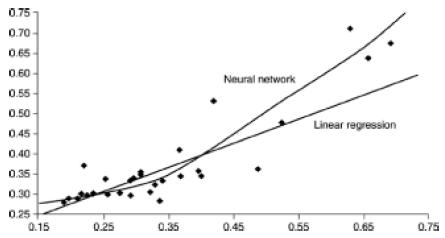
\includegraphics[width=.7\textwidth]{imagem/figura6.png}
	% Caption centralizada
	\captionsetup{justification=centering}
	% Caption e fonte
	\\
	\small{Fonte: \cite{Pyle1999}.}
	\label{img:regressao}
\end{figure}

% Nome do capitulo
\chapter{Data Warehouse}
% Label para referenciar
\label{cap:dw}
% Diminuir espacamento entre titulo e texto
\vspace{-1.9cm}

% Texto do capitulo
\ac{DW}, ou armaz�m de dados, consolidam dados em espa�os multidimensionais. Eles podem ser vistos como uma etapa importante para a minera��o de dados. Al�m disso prov� integra��o com ferramentas \ac{OLAP} para an�lise interativa dos dados. O DW prov� ferramentas e arquitetura para que os respons�veis pelos neg�cios organizem, entendam e usem seus dados para tomarem decis�es estrat�gicas \cite{Etal.Han2005}.

O \textit{Data Warehouse} � orientado a um assunto espec�fico, integrado, n�o vol�til e com tempo variante para o suporte do processo de tomada de decis�es. Ele � organizado em torno de um objetivo principal, como rela��es nas vendas, ao inv�s de se concentrar em opera��es e transa��es di�rias. Dizemos que o DW � integrado por ser constru�do atrav�s de m�ltiplas fontes, como banco de dados relacionais diversos, planilhas e outros sistemas. Refere-se a um banco de dados que � mantido separado do banco de dados das opera��es organizacionais. Ent�o n�o requer processamento de transa��es, \textit{backups} cont�nuos e mecanismos de controle. Basicamente o DW realiza apenas duas opera��es: carregamento inicial e acesso aos dados. Todas as informa��es armazenadas dizem respeito a um per�odo de tempo definido normalmente entre 5 a 10 anos \cite{Etal.Han2005}.

Para permitir modelar e visualizar as m�ltiplas dimens�es do DW utiliza-se os CUBOS. Os Cubos s�o definidos por dimens�es e fato. O fato significa o tema do modelo, representado por uma tabela principal. J� as dimens�es s�o as entidades que dizem respeito aquilo que a organiza��o deseja armazenar, as tabelas ao redor do fato. Apesar de pensarmos no Cubo como uma estrutura 3D, no \textit{data warehousing} ele � n-dimensional. � poss�vel ver no cubo, por exemplo, dados de acordo com o tempo, item, localiza��o e fornecedor. Ou seja, uma visualiza��o 4D \cite{Etal.Han2005}.

Assim como o fato e as dimens�es, a hierarquia � uma caracter�stica do DW. O conceito de hierarquia define a sequ�ncia do mapeamento dos mais baixos aos mais altos conceitos. Um exemplo dessa hierarquia pode ser visto na dimens�o Tempo, onde tem-se as horas como conceitos mais baixos e os anos como conceitos mais altos. Essa hierarquia prov� ao usu�rios a flexibilidade de acordo com suas necessidades \cite{Etal.Han2005}.

Para o modelo entidade-relacionamento � desenhado  um modelo de rela��es entre as entidades. Entretanto, para o DW � utilizado um modelo multidimensional como o estrela, floco de neve ou mesmo constela��o. O esquema estrela cont�m uma grande tabela central, o fato, com uma s�rie de tabelas menores em volta, as dimens�es. O esquema floco de neve � uma varia��o do esquema estrela, por�m as tabelas de dimens�es s�o normalizadas. Ent�o as tabelas existentes s�o divididas  resultando em uma forma final similar a um floco de neve. A maior diferen�a entre esses dois esquemas � que o segundo modelo reduz as redund�ncias no banco, reduzindo tamb�m o espa�o de armazenamento. Por�m apesar dessa redu��o, esse esquema perde performance por ter que executar mais \textit{joins} em suas consultas. O �ltimo esquema, constela��o, especifica duas tabelas fatos. Assim � permitido �s dimens�es serem compartilhadas entre os fatos \cite{Etal.Han2005}.

A arquitetura de um DW pode ser representada de acordo com a Figura \ref{fig:arquiteturadw}. No centro da imagem est� o reposit�rio, composto pelos dados e metadados. Para alimentar esse banco s�o usadas fontes externas, ferramentas de \textit{back-end} e utilit�rias. Essas ferramentas executam a extra��o dos dados das diferentes fontes, assim como sua limpeza e transforma��o. Essa camada � conhecida como Extra��o, Transforma��o e Carga, do ingl�s \ac{ETL}. A Camada \ac{OLAP} mapeia as opera��es nos dados multidimensionais. No topo da arquitetura a camada do cliente, \textit{front-end}. Essa camada cont�m as ferramentas de consultas, relat�rios, an�lises e minera��o de dados \cite{Etal.Han2005}.
 
% Figura
\begin{figure}[ht]
	\caption{\textbf{Arquitetura de um Data Warehouse} (Tradu��o por Dayana Viana)}
	\centering
	% Alterar espa�amentos antes e depois do caption
	\setlength{\abovecaptionskip}{0pt}
	\setlength{\belowcaptionskip}{0pt}
	% Arquivo da figura
	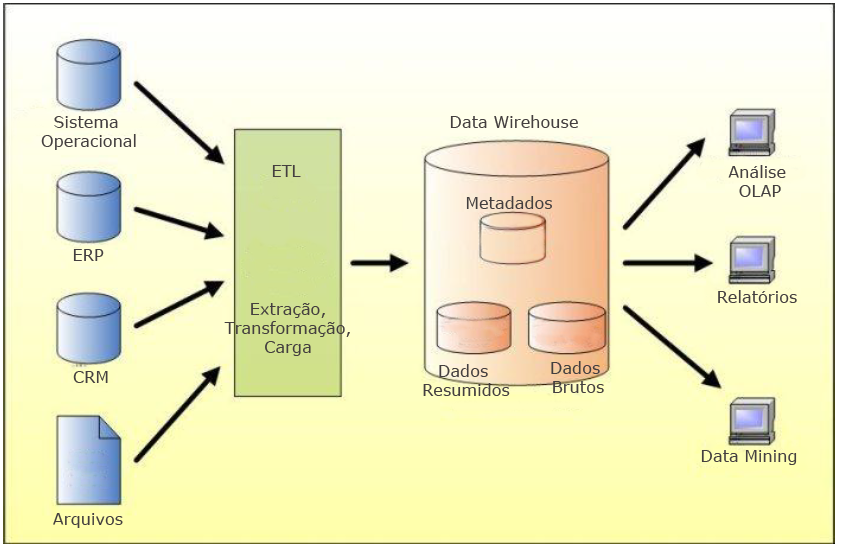
\includegraphics[width=.9\textwidth]{imagem/figura10.png}
	% Caption centralizada
	\captionsetup{justification=centering}
	% Caption e fonte
	\\
	\small{Fonte: \cite{Reboucas}.}
	\label{fig:arquiteturadw}
\end{figure}

As informa��es processadas s�o baseadas em consultas. Apesar de retornarem informa��es �teis, refletem diretamente as informa��es armazenadas. Ou seja, n�o refletem os padr�es do banco de dados. Uma vez que a minera��o de dados envolve uma an�lise mais profunda do que a OLAP, a utiliza��o da minera��o permitir� aplica��es mais amplas do conhecimento obtido.



% Nome do capitulo
\chapter{SQL Server}
% Label para referenciar
\label{cap:sqlserver}
% Diminuir espacamento entre titulo e texto
\vspace{-1.9cm}

% Texto do capitulo
Um banco de dados � um sistema computacional para armazenamento de registros. Ou seja, � um reposit�rio de dados que pode at� mesmo ser comparado a um arm�rio de arquivos. Os dados armazenados representam qualquer coisa que tenha sentido � organiza��o. S�o tudo aquilo que � necess�rio para auxiliar a tomada de decis�es. Intermediando o banco de dados e seus usu�rios existe uma camada conhecida como \ac{SGBD}.  Todas as altera��es solicitadas ao banco de dados s�o realizadas pelo SGBD (Figura \ref{fig:sgbd}). Uma grande vantagem desse ambiente � que o sistema de banco de dados proporciona um controle centralizado dos dados \cite{Date2000}. Basicamente podemos aplicar o banco de dados em qualquer cen�rio que necessite armazenar informa��es como, por exemplo, em softwares de gest�o e \textit{Data Warehouse}. 

% Figura
\begin{figure}[ht]
	\caption{\textbf{Composi��o do Banco de Dados}}
	\centering
	% Alterar espa�amentos antes e depois do caption
	\setlength{\abovecaptionskip}{0pt}
	\setlength{\belowcaptionskip}{0pt}
	% Arquivo da figura
	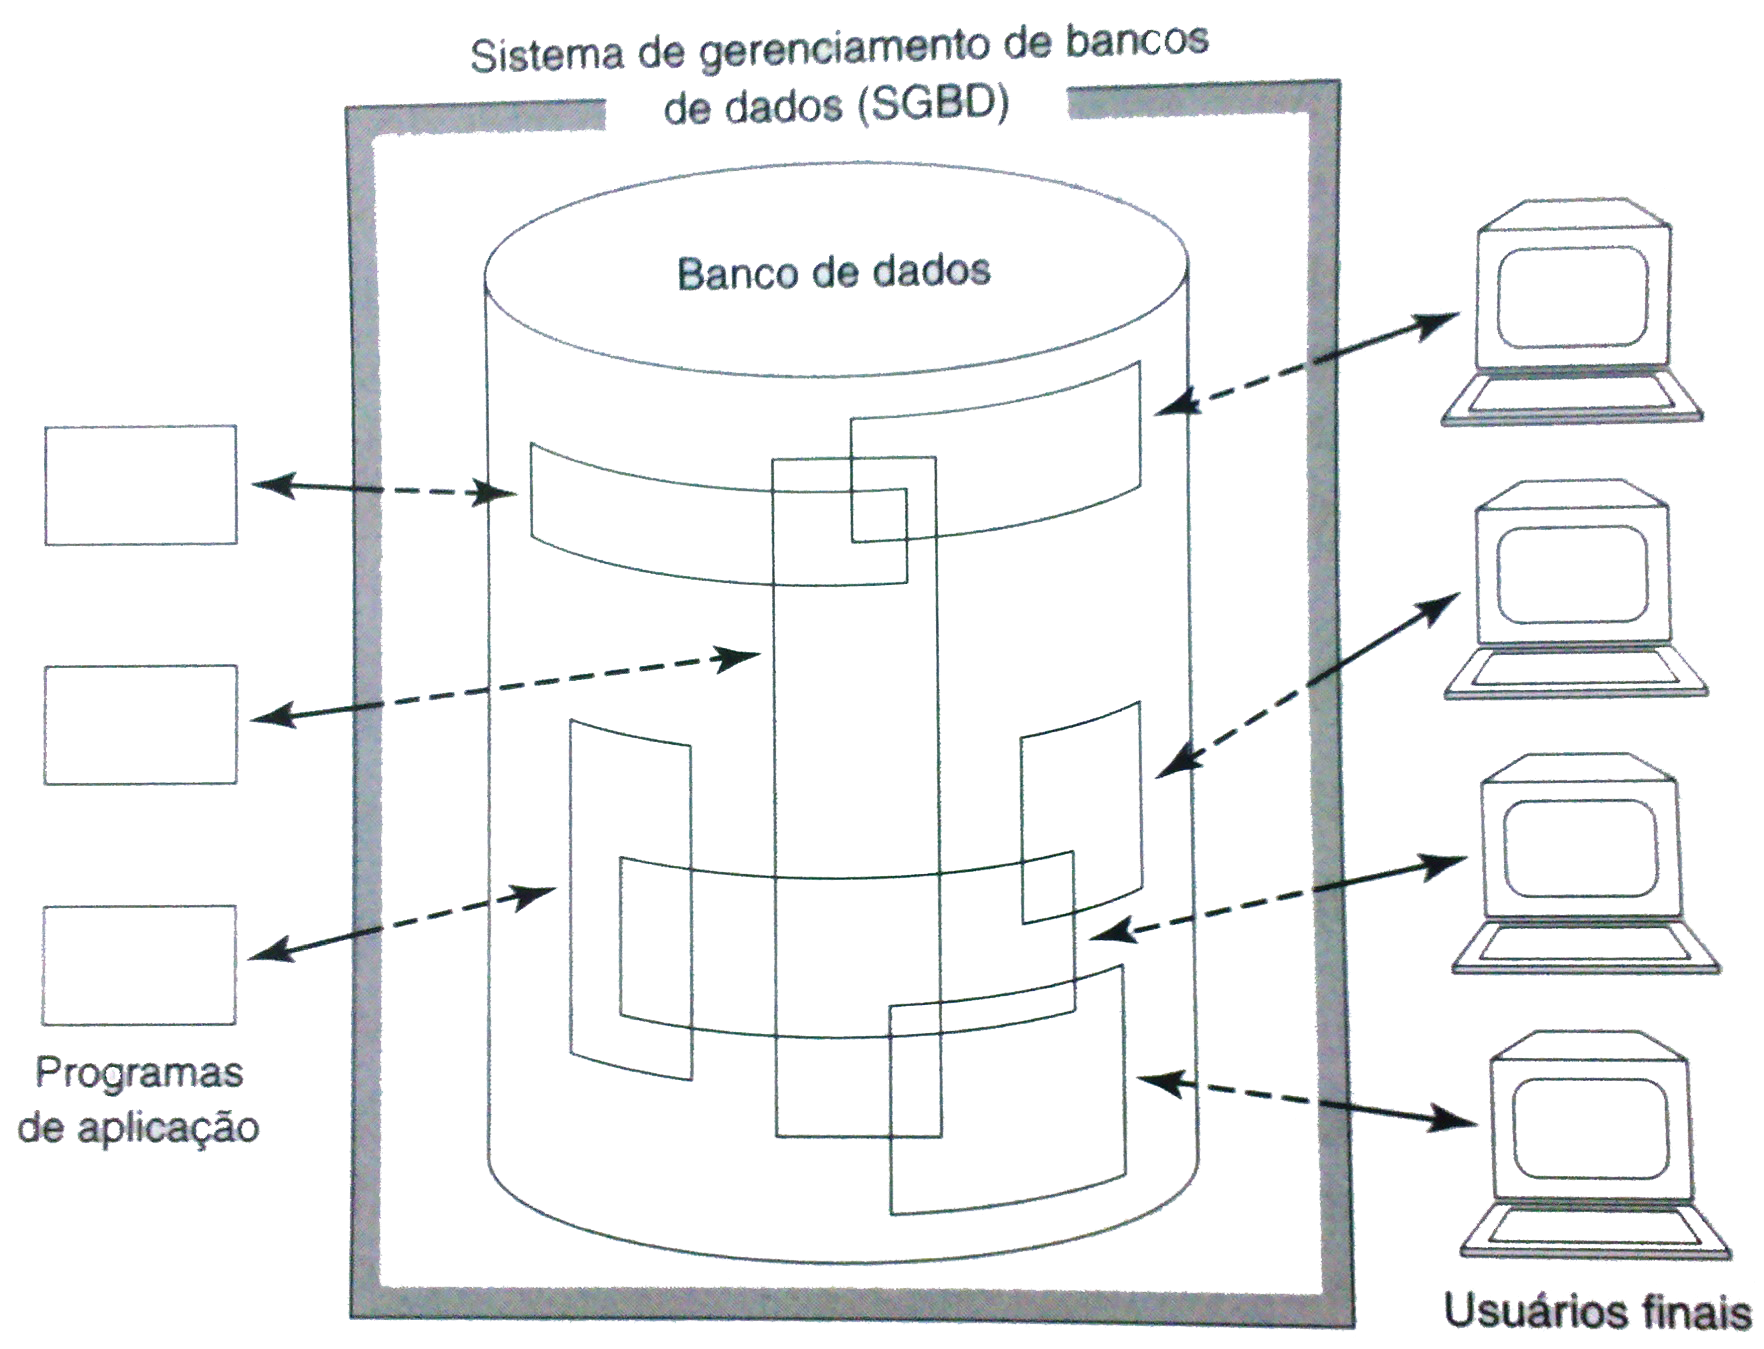
\includegraphics[width=.7\textwidth]{imagem/figura8.png}
	% Caption centralizada
	\captionsetup{justification=centering}
	% Caption e fonte
	\\
	\small{Fonte: \cite{Date2000}.}
	\label{fig:sgbd}
\end{figure}

O SQL Server � mais que um banco de dados, ele � uma plataforma de dados. Al�m de persistir os dados ele tamb�m possui todas as ferramentas necess�rias para prepara��o de um Sistema de \ac{BI}. Esse tipo de sistema facilita a transforma��o dos dados em informa��es para auxiliar as tomadas de decis�es. Os componentes do SQL Server s�o o \textit{SQL Server Management Studio} e \textit{SQL Server Bussiness Inteligence Development Studio} incluindo \textit{Reporting Services}, \textit{Analysis Services} e \textit{Integration Services}. A interface mais utilizada da plataforma SQL Server � o \textit{SQL Server Management Studio}, um software com foco na administra��o do banco de dados.  A outra interface do produto, usada com foco no desenvolvimento, � o\textit{SQL Server Bussiness Inteligence Development Studio}. Essa interface inclui outras ferramentas (Figura \ref{fig:sqldevstudio}) como por exemplo geradores de relat�rios (\textit{Reporting Services}), operador de banco de dados multidimensionais (\textit{Analysis Services}) e ferramenta ETL (\textit{Integration Services}).

% Figura
\begin{figure}[ht]
	\caption{\textbf{Estruturas do SQL Server}}
	\centering
	% Alterar espa�amentos antes e depois do caption
	\setlength{\abovecaptionskip}{0pt}
	\setlength{\belowcaptionskip}{0pt}
	% Arquivo da figura
	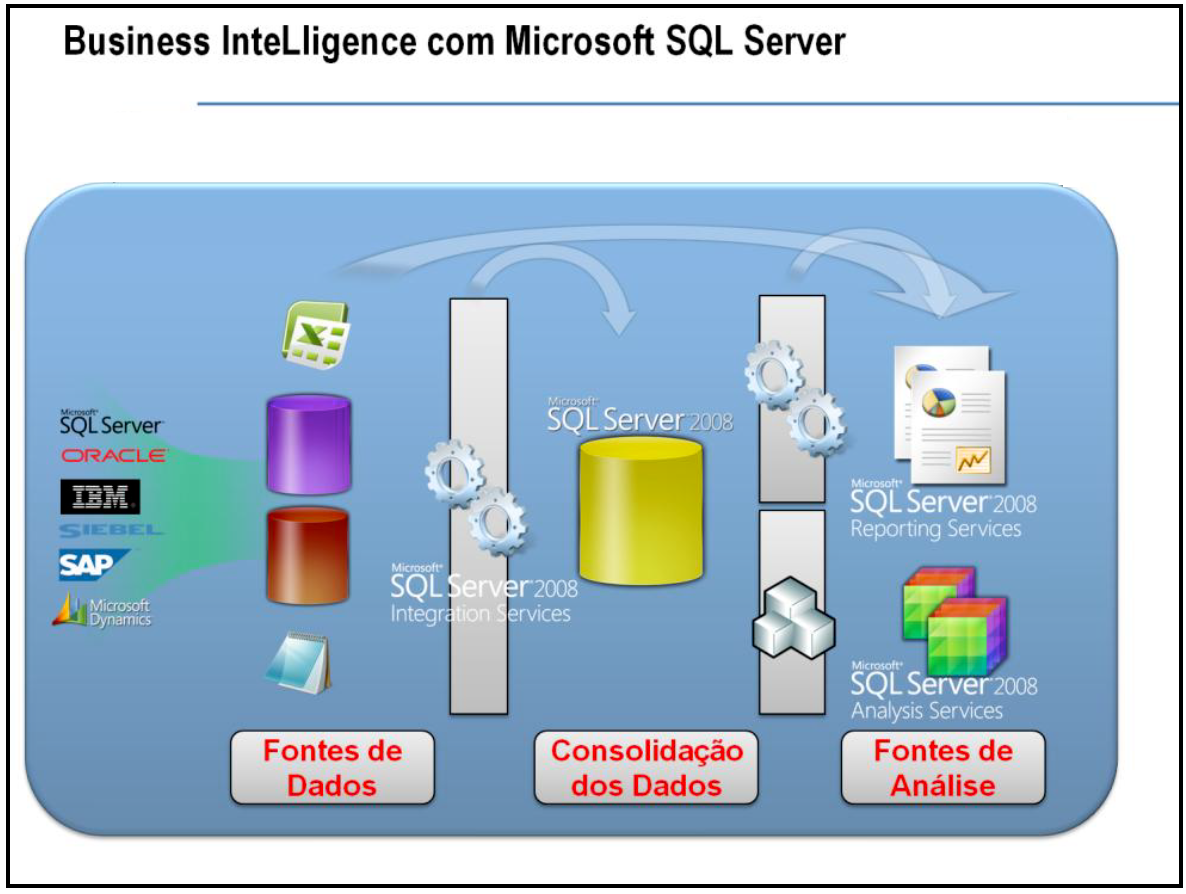
\includegraphics[width=.7\textwidth]{imagem/figura9.png}
	% Caption centralizada
	\captionsetup{justification=centering}
	% Caption e fonte
	\\
	\small{Fonte: Tutorial \ac{S2B} - Componentes do Banco de Dados.}
	\label{fig:sqldevstudio}
\end{figure}

O \textit{Analysis Services} � uma ferramenta de \textit{Data Mining} para apoiar as estrat�gias. A ferramenta possibilita obten��o de informa��es importantes que podem auxiliar no processo decis�rio da institui��o. O \textit{Analysis Services} oferece diversas solu��es para implantar banco de dados anal�ticos usados para apoio � decis�o em aplicativos de BI e at� mesmo Excel. A partir de dados hist�ricos j� coletados s�o criados metadados que permitem medir, manipular e comparar esses dados. A partir da cria��o de um modelo dos dados, ele � ent�o implantado em um servidor do \textit{Analysis Services} como um banco de dados e disponibilizado para conex�es externas como Excel ou outras ferramentas \cite{MSDNas}.

Uma op��o de ferramenta de apresenta��o para analisar os dados persistentes no \textit{Analysis Services} � o Microsoft Office Excel. O Excel al�m de criar tabelas e realizar c�lculos o � tamb�m um software de an�lise de dados. Para isso necessita do \textit{Data Mining Add-in}, uma exten��o da ferramenta que � instalada separadamente. Ap�s a instala��o deve-se conectar a uma fonte de dados de Processamento Anal�tico Online (OLAP), disponibilizada pelo SQL Server. Atrav�s dessa conex�o � poss�vel exibir os dados como relat�rio de tabelas ou gr�ficos din�micos \cite{OfficeOLAP}.




% Nome do capitulo
\chapter{Microdados do Censo da Educa��o Superior}
% Label para referenciar
\label{cap:microdados}
% Diminuir espacamento entre titulo e texto
\vspace{-1.9cm}

% Texto do capitulo
Desde 1988, nossa Constitui��o da Rep�blica Federativa disp�s a necessidade de armazenar dados estat�sticos. As informa��es obtidas atrav�s desses dados contribuem para nortear pol�ticas p�blicas e educacionais. Essa necessidade foi refor�ada pelo art. 9� da Lei n� 9.394 em 1996. Surgiram ent�o decretos que culminaram na cria��o do Decreto no 6.425 em 2008. Esse decreto prev� a obrigatoriedade de Institui��es de Ensino Superior (IES) para responderem ao Censo \cite{Inep2012}.

Anualmente � realizado pelo \ac{Inep} uma coleta dos dados sobre a educa��o superior. Um Question�rio � enviado para as IES responderem perguntas sobre seus cursos, alunos e sua pr�pria estrutura (Decreto no 6.425). Os dados coletados nos question�rios re�nem informa��es sobre os diversos cursos oferecidos, vagas, inscri��es, evas�es, etc. Esses dados s�o ent�o disponibilizados � sociedade em geral para manipula��es estat�sticas, por�m mantendo sigilo quanto as informa��es dos alunos e institui��es. Com os dados podemos obter informa��es como a situa��o atual e as tend�ncias das IES e da comunidade \cite{Inep2011}.
 
Os microdados coletados ficam dispon�veis no portal do Inep: <http://portal.inep.gov- .br/basica-levantamentos-acessar> e s�o organizados em arquivos separados por ano. Os formatos para download s�o Texto ASCII, que permite a leitura por diversos softwares, e inputs para a leitura utilizando softwares SAS e SPSS. Para esse trabalho a base de dados utilizada foi manipulada e disponibilizada em formato excel, com as informa��es acumuladas entre o per�odo de 2001 a 2008.

Os dados obtidos est�o organizados em 7 planilhas: Turno, Munic�pio, Tipo Curso, Institui��o, Categoria Administrativa, Curso e Dados MG. A planilha Turno armazena os turnos dispon�veis dos cursos, s�o eles Diurno e Noturno. Em Munic�pio temos listados os 853 munic�pios de Minas Gerais. Para Tipo de Curso, os dados s�o divididos entre Gradua��o e cursos Tecn�logos. Em Institui��es temos uma lista de 2217 estabelecimentos onde o nome dos mesmos foi preservado em sigilo. Categoria Administrativa classifica as institui��es como P�blicas ou Privadas. Na planilha Curso, al�m da listagem de 600 nomes de cursos, temos tamb�m informa��es sobre a �rea de cada curso. Finalmente em Dados MG � feita refer�ncia a todas planilhas citadas anteriormente, ordenadas por ano e semestre, juntamente com mais alguns dados adicionais como Ano de In�cio do Curso, Quantidade de Vagas, Quantidade de Inscritos, Quantidade de Calouros, Quantidade de Transfer�ncia Interna, Quantidade de Transfer�ncia Externa, Quantidade de Portador de Diploma, Quantidade de Reingresso, Quantidade de Outros Ingressos, Quantidade de Matriculados, Quantidade de Concluintes, Quantidade de Matr�culas Trancadas, Quantidade de Desistentes, Quantidade que Mudou de Curso e Quantidade que Mudou de Institui��o.

Observando essas planilhas � poss�vel abstrair um modelo de dados, representado pela Figura \ref{fig:modelodados}.

% Figura
\begin{figure}[ht]
	\caption{\textbf{Modelo de Dados}}
	\centering
	% Alterar espa�amentos antes e depois do caption
	\setlength{\abovecaptionskip}{0pt}
	\setlength{\belowcaptionskip}{0pt}
	% Arquivo da figura
	\includegraphics[width=1\textwidth]{imagem/modeloBD.png}
	% Caption centralizada
	\captionsetup{justification=centering}
	% Caption e fonte
	\\
	\small{Fonte: Cria��o da autora.}
	\label{fig:modelodados}
\end{figure}
%
\capitulo{METODOLOGIA}

\iniciocapitulo
A resolução deste trabalho está dividida nas seguintes partes instalação do ambiente, análise e algorítimo.\par

A implementação do sistema se deve primeiramente a configuração do ambiente para o início do desenvolvimento os seguintes passos devem ser tomados para que o ambiente seja reproduzido novamente. Primeiramente deve se instalar o SGBD PostgreSQL, logo em seguida deve se instalar o JAVA 7 em sua maquina, para validar a instalação deve-se executar o seguinte comando "java -version && javac -version" a mensagem descrita na figura XX deve ser mostrada.

\begin{figure}[!htb]
\caption[Versão Java]{Versão Java}
\label{fig:figura2}
\centering
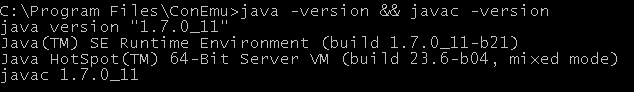
\includegraphics[scale=0.8]{imagens/mensagemJava.png}
\\ \textbf{\footnotesize Fonte: Autor}
\end{figure}


Após a instalação do java deve-se instalar o framework Play! seguindo os passos encontrados no site \cite{play} para validar a instalação do Play! deve se executar o comando "play version" e o \textit{prompt} de comando deve retornar a mensagem conforme mostra a figura figura XX.

\begin{figure}[!htb]
\caption[Versão Framework]{Versão Framework}
\label{fig:figura2}
\centering
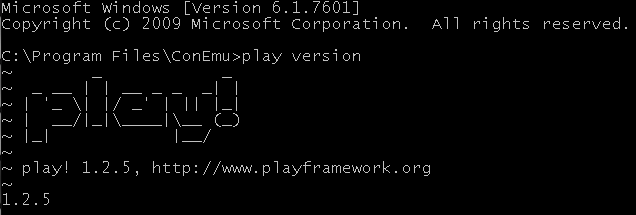
\includegraphics[scale=0.8]{imagens/mensagemPlay.png}
\\ \textbf{\footnotesize Fonte: Autor}
\end{figure}

Uma vez que o ambiente já está configurado devemos inciar um projeto no framework instalado através do comando "play new nomeDoProjeto", a partir dai é possível escolher IDE que será utilizada.

Foi criado um \textit{script} para criação do banco de dados e população inicial das informações como, prédios, salas, turnos, horários, e disciplinas com informações que são necessárias em todo inicio de semestre na instituição de ensino escolhida.

PQ do algoritimo genetico
segundo renand dupas a escolha de algoritimoes geneticos se dá através de uma comparação com outras técnicas e através disso de uma evidenciação das vantagens de sua utilização , logo o algoritimo genetico foi escolhido para este trabalho.

População inicial = --UMA NOVA ABORDAGEM PARA AUMENTAR A DIVERSIDADE.pdf

modelo matematico ----APLICAÇÃO DE MODELO MATEMÁTICO, ABORDAGEM HEURÍSTICA E MÉTODO MISTO NA OTIMIZAÇÃO DA PROGRAMAÇÃO DE HORÁRIO DOS PROFESSORESTURMAS.pdf

restrições do problema e modelo matematico http://www.dcc.ufla.br/infocomp/artigos/v4.3/art08.pdf

Foi realizada uma análise dos requisistos atravez de entrevista com o steakholder, após as entrevistas a modelagem de dados foi realizada de acordo com a demanda do projeto, para o desenvolvimento destes diagramas foi utilizadas a UML (Universal Modeling Language). Os seguintes diagramas foram desenhados, diagrama de caso de uso, diagrama de classe e diagrama de entidade relacionamento. Foram escolhidos os seguintes diagramas para que o sistema tenha uma documentação minima tendo em vista que o foco do trabalho é a resolução do problema de timetable através da utilização do algoritimo genetico.

Por se tratar de um sistema complexo, antes de iniciar a implementação do sistema
fez-se necessário a sua modelagem. Segundo Elmasri & Navathe (2005) as metodologias
de modelagem de dados de objetos como UML (Universal Modeling Language –
Linguagem de Modelagem Universal) estão se tornando cada vez mais populares no
projeto e engenharia de software. Essas metodologias vão além do projeto de um banco de
dados, especificando o projeto detalhado dos módulos de software e suas interações,
utilizando vários tipos de diagramas.\par

\secao{Ferramentas Utilizadas}

Este trabalho conta com a utilização de tecnologias proprias para o desenvolvimento de sistemas web, foram utilizadas as seguintes ferramentas: Para SGBD foi o utilizado PostgreSQL; No back-end foi utilizado Java e o \textit{framework Play!}; No front-end as tecnologias utilizadas foram HTML, CSS, JavaScript e \textit{framework AngularJS} e a IDE utilizada \textit{Eclipse}.\par



\subsecao{Sistema de Gerenciamento de Banco de Dados}

O SGBD escolhido foi o PostgreSQL pelo fato de ser uma ferramenta open-source e que trabalha perfeitamente com o framework escolhido Play!, uma vez que utilizado em projetos anteriores não foram apresentados conflitos entre o framework e o SGBD. A seguir pode ser notar que é uma ferramenta robusta e que tem visão no mercado internacional.\par

O PostgreSQL é um poderoso sistema gerenciador de banco de dados objeto-relacional de código aberto.  Tem mais de 15 anos de desenvolvimento ativo e uma arquitetura que comprovadamente ganhou forte reputação de confiabilidade, integridade de dados e conformidade a padrões.  Roda em todos os grandes sistemas operacionais. É totalmente compatível com ACID, tem suporte completo a chaves estrangeiras, junções (JOINs), visões, gatilhos e procedimentos armazenados (em múltiplas linguagens).  Inclui a maior parte dos tipos de dados do ISO SQL:1999, incluindo INTEGER, NUMERIC, BOOLEAN, CHAR, VARCHAR, DATE, INTERVAL, e TIMESTAMP.  Suporta também o armazenamento de objetos binários, incluindo figuras, sons ou vídeos.  Possui interfaces nativas de programação para C/C++, Java, .Net, Perl, Python, Ruby, Tcl, ODBC, entre outros, e uma excepcional documentação.\cite{postgresql}



Para a resolução do problema de timetable foi escolhido o algoritimo genetico, a escolha do algoritimo foi devida a grande utilização do mesmo para resolução de problemas do tipo NP-dificil que foram encontrados na literatura.
\par




\subsecao{Ferramentas Back-end}

Foi escolhida uma linguagem de programação Java por ser orientada a objeto. Tambem foi escolhido o \textit{Play! framework}, para que o desenvolvimento aconteça de forma mais rápida, fácil e eficiente.\par

%Java
Java foi criada pela Sun Microsystems para desenvolver inovações tecnológicas em 1992, time liderado por James Gosling. O Java utiliza do conceito de máquina virtual, onde existe, entre o sistema operacional e a aplicação, uma camada extra responsável por \"traduzir\" - mas não apenas isso - o que sua aplicação deseja fazer para as respectivas chamadas do sistema operacional, onde ela está rodando no momento. Sua aplicação roda sem nenhum envolvimento com o sistema operacional, sempre conversando apenas com a JVM - Java Virtual Machine \cite{caelum}.\par

Em 2009 a Oracle comprou a Sun, fortalecendo a marca. A Oracle sempre foi, junto com a IBM, uma das empresas que mais investiram e fizeram negócios através do uso da plataforma Java. Em 2011 surge a versão Java 7 com algumas pequenas mudanças na linguagem \cite{caelum}.\par

%-----Play! Framework

The Play! É um moderno framework MVC de alta produtividade, que utiliza Java e Scala para o desenvolvimento web, open-source , utiliza templates, hibernate e JUnit  em sua arquitetura. Existe duas versões do framework Play! 1 e Play2! este trabalho utiliza a versão 1 do framework\cite{playframework}.\par


\subsecao{Ferramentas Front-end}

As ferramentes de Front-end descritas abaixo, foram escolhidas devida a gande utilização na web grande parte dos sites contem HTML, CSS ou JavaScript em algum trexo de seu código, foi escolhido tambem o framework AngularJS para que o desenvolvimento ocorra de maneira agil e mais rapida.\par

%HTML
HTML que é defindo por (\textit{HyperText Markup Language}) ou linguagem de marcação, é uma linguagem que é utilizada no desenvolvimento de paginas web \cite{html}.\par

%css
Cascading Style Sheets (CSS) é uma tecnologia utilizada para adicionar estilos como cores, fontes, espaçamentos em documentos escritos em uma linguagem de marcação como exemplo o HTML \cite{css}.\par

%JAVASCRIPT

JavaScript é uma linguagem de script utilizada no desenvolvimento de paginas na web, atualmente é a principal linguagem para programação client-side em navegadores web. Todas as paginas de HTML modernas estão usando JavaScript para adicionar funcionalidades e para se comunicar com os webServers\cite{javascript}.\par

Angularjs é um \textit{framework JavaScript} construido e mantido pelo grupo de engenheiros do Google, ele usa o HTML como uma \textit{template engine}, tudo isso no intuito de fornecer uma solução completa para o cliente-side de sua aplicação. Além disso tem total compatibilidade com as bibliotecas javascript mais utilizadas, como jQuery. É um novo conceito para desenvolvimento de web apps client-site.\cite{angularjs}\par

\subsecao{IDE}

O Eclipse é uma IDE (\textit{integrated development environment}). Diferente de uma RAD(\textit{Rapid Application Development}), onde o objetivo é desenvolver o mais rápido possível através do arrastar-e-soltar do mouse, onde montanhas de código são gerados em background, uma IDE te auxilia no desenvolvimento, evitando se intrometer e fazer muita mágica \cite{caelum}.\par

O Eclipse é a IDE líder de mercado. Formada por um consórcio liderado pela IBM, possui seu código livre. A última versão é a 4.3, mas com qualquer versão posterior a do 3.1 você terá suporte ao Java 5, 6 e 7 \cite{caelum}.\par

Está IDE foi escolhida devido ao grande reconhecimento mundial, por sua eficiencia ao se trabalhar com a linguagem de programação Java, por ser open-source e pela existencia de varias ferramentas criadas pela comunidade, para o auxilio no desenvolvimento de softwares.\par
% Nome do capitulo
\chapter{Desenvolvimento}
% Label para referenciar
\label{cap:desenvolvimento}
% Diminuir espacamento entre titulo e texto
\vspace{-1.9cm}

% Texto do capitulo

% Nome do subcapitulo
\section{Processo KDD}
% Label para referenciar
\vspace{0.4cm}
% Texto do subcapitulo
Este cap�tulo tem como objetivo apresentar o processo de KDD que foi aplicado sobre os Microdados do Censo da Educa��o Superior. Ser� explicado como foi executada cada etapa desse processo. 

% Nome do capitulo
\subsection{Sele��o de Dados}
% Label para referenciar
\vspace{0.3cm}
% Texto do capitulo
Os microdados do Censo da Educa��o Superior apresentam informa��es coletadas por todo o pa�s desde 1995. Por�m nesse trabalho delimitou-se o escopo nos dados sobre Minas Gerais entre o per�odo de 2001 a 2008. O \ac{GTI} j� disponibiliza uma base, em formato Excel, com as informa��es do portal do Inep agrupadas dentro desse intervalo temporal. O que auxilia no processo de sele��o, pois originalmente os dados de cada ano s�o disponibilizados separadamente. Apesar de trabalhar nessa base selecionada pelo GTI, dentro dela tem ainda um foco maior sobre as informa��es relacionadas � PUC Minas e ao curso de Sistemas de Informa��o da PUC Minas.

% Nome do capitulo
\subsection{Pr�-Processamento}
% Label para referenciar
\vspace{0.3cm}
% Texto do capitulo
Em rela��o aos relacionamentos, os dados trabalhados j� estavam organizados de forma eficiente. Garantem agilidade e esfor�o reduzido nas an�lises das consultas por manter os campos que ser�o relacionados com o tipo inteiro.

O maior problema encontrado na base de dados foi a aus�ncia de informa��o na planilha Dados\_MG. Aplicando a fun��o CONTAR.VAZIO do Excel, percebe-se que n�o havia falhas entre as colunas cujo os c�digos se relacionam com as outras planilhas. Por�m, observando as outras colunas, com os dados relativos �s quantidades foi encontrado uma m�dia de 53\% dos campos vazios.

Substituir os valores ausentes em um conjunto de dados � muito importante. Os valores ausentes devem ser substitu�dos de forma que os valores inseridos n�o modifiquem os padr�es j� existentes nos dados \cite{Pyle1999}. Pensando nisso e observando que o tipo de dados das colunas com valores ausentes eram n�meros inteiros positivos, foi ent�o preenchido estrategicamente os campos com o valor zero. Assim os padr�es das quantidades atuais n�o foram alterados.

Nessa etapa foi identificado o c�digo da Institui��o foco do trabalho. Foi alterado o nome de ``Institui��o 1934'' para ``PUC Minas''. Para identificar a Institui��o foram filtrados os dados selecionando o Munic�pio de Arcos (c�digo 310420) e o curso de Sistemas de Informa��o (c�digo 518). Como resultado tivemos apenas o c�digo de institui��o 1934, indicando a comprova��o do fato de que apenas a PUC Minas tem o curso de Sistemas de Informa��o no munic�pio de Arcos e que seu c�digo nessa base � o 1934.

Foram tamb�m criados dois novos campos: Ano e Semestre, Afim de suprir a necessidade de an�lises anuais. A base de dados original apresenta esses valores juntos limitando assim as an�lises por semestre. 

% Nome do capitulo
\subsection{Transforma��o}
% Label para referenciar
\vspace{0.3cm}
% Texto do capitulo
Nessa etapa foi realizado o enriquecimento dos dados. Analisando, pode-se perceber que existem informa��es ocultas que poderiam ser explicitadas. Foram adicionadas ent�o quatro novas colunas ao documento afim de agregar valor ao trabalho. Essas colunas informam a Quantidades de Ingressantes, Quantidades de Evas�o, Rela��o Candidato Vaga e Taxa de Ocupa��o.

Quantidade de Ingressantes ($Qt\_{Ing}$) � obtida a partir do somat�rios das colunas de Quantidade de Calouros ($Qt\_{Cal}$), Quantidade de Transfer�ncia Interna ($Qt\_{TransfInt}$), Quantidade de Transfer�ncia Externa ($Qt\_{TransfExt}$), Quantidade de Reingresso ($Qt\_{Reing}$) e Quantidade de Outros Ingressos ($Qt\_{Outros}$), conforme equa��o a seguir. 

\begin{equation*}
	$Qt_{Ing} = Qt_{Cal} + Qt_{TransfInt} + Qt_{TransfExt} + Qt_{Reing} + Qt_{Outros}$
\end{equation*}

A Quantidade de Evas�o ($Qt\_{Ev}$) � obtida a partir do somat�rio das colunas Quantidade de Matr�culas Trancadas ($Qt\_{Tranc}$), Quantidade de Desistentes ($Qt\_{Deist}$), Quantidade que Mudou de Curso ($Qt\_{MudCurso}$) e Quantidade que Mudou de Institui��o ($Qt\_{MudInst}$).

\begin{equation*}
	$Qt_{Ev} = Qt_{Tranc} + Qt_{Deist} + Qt_{MudCurso} + Qt_{MudInst}$
\end{equation*}

A rela��o Candidato Vaga ($Cand\_vaga$) � obtida dividindo-se a Quantidade de Inscritos ($Qt\_{Insc}$) pela Quantidade de Vagas ($Qt\_{Vagas}$). 

\begin{equation*}
 	$Cand\_vaga = \frac{Qt_{Insc}}{Qt_{Vagas}}$
\end{equation*}

Por �ltimo, a Taxa de Ocupa��o ($Qt\_{TxOcup}$) � representada em porcentagem e � o resultado da divis�o entre a soma da Quantidade de Calouros ($Qt\_{Cal}$), Quantidade de Transfer�ncia Interna ($Qt\_{TransfInt}$), Quantidade de Transfer�ncia Externa ($Qt\_{TransfExt}$), Quantidade de Reingresso ($Qt\_{Reing}$), e Quantidade de Outros Ingressos ($Qt\_{Outros}$) sobre a Quantidade de Vagas ($Qt\_{Vagas}$).

\begin{equation*}
	$Qt_{TxOcup} = \frac{Qt_{Cal} + Qt_{TransfInt} + Qt_{TransfExt} + Qt_{Reing} + Qt_{Outros}}{Qt_{Vagas}}$
\end{equation*}

Ap�s todo esse processo chegou-se ao modelo de dados representado pela Figura \ref{img:modelofinal}. Com o arquivo fonte tratado, foi feita a importa��o para o SQL Server 2012. Ap�s isso o cubo foi criado utilizando-se o \textit{Analysis Services}.

% Figura
\ \ \ 
\begin{figure}[ht]
	\caption{\textbf{Modelo de Dados modificado}}
	\centering
	% Alterar espa�amentos antes e depois do caption
	\setlength{\abovecaptionskip}{0pt}
	\setlength{\belowcaptionskip}{0pt}
	% Arquivo da figura
	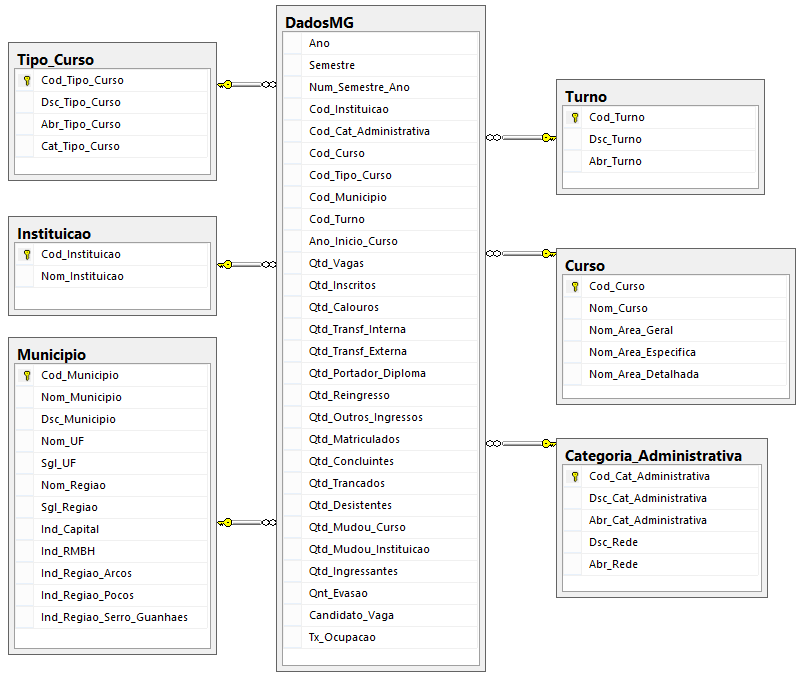
\includegraphics[width=1\textwidth]{imagem/modelofinal.png}
	% Caption centralizada
	\captionsetup{justification=centering}
	% Caption e fonte
	\\
	\small{Fonte: Cria��o da autora.}
	\label{img:modelofinal}
\end{figure}

% Nome do capitulo
\subsection{Minera��o de Dados}
% Label para referenciar
\vspace{0.3cm}
% Texto do capitulo
Na Minera��o de Dados foi utilizado o Excel 2010 juntamente com o \textit{Data Mining Add-In} para SQL Server 2012. Com o Excel � poss�vel fazer uma An�lise Descritiva dos Dados, ou seja, apresentar o que os dados atuais trazem de informa��es. O uso do \textit{Add-In} viabiliza a an�lise de modelos aplicando os algor�timos de Minera��o de Dados e visualizando os resultados em forma de gr�ficos. 

Para gerar as An�lises Descritivas dos Dados foi realizada uma conex�o entre o Excel e o banco de dados. Ent�o cria-se Gr�ficos Din�micos, utilizando essa conex�o, selecionando os dados nas quais deseja que a an�lise seja feita. Nas An�lises de Modelo de Dados a conex�o � realizada com o \textit{Analysis Services}, assim s�o aplicados os algoritmos ao cubo criado anteriormente. O \textit{Add-In} possui diversos m�todos que podemos utilizar para realizar as an�lises (Figura \ref{img:addin}), por�m foram utilizados apenas os m�todos de prever, detectar categorias, an�lise de influ�ncias e an�lise da cesta de compras.

% Figura
\begin{figure}[ht]
	\caption{\textbf{Ferramenta de An�lise de Tabela}}
	\centering
	% Alterar espa�amentos antes e depois do caption
	\setlength{\abovecaptionskip}{0pt}
	\setlength{\belowcaptionskip}{0pt}
	% Arquivo da figura
	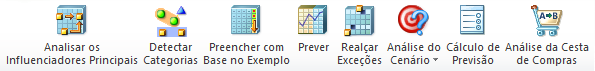
\includegraphics[width=1\textwidth]{imagem/addin.png}
	% Caption centralizada
	\captionsetup{justification=centering}
	% Caption e fonte
	\\
	\small{Fonte: Add-in Excel 2010.}
	\label{img:addin}
\end{figure}

O m�todo Prever executa a previs�o dos valores das colunas que forem selecionadas. Como padr�o a quantidade de unidade de tempo a ser prevista � 5, por�m esse valor pode ser modificado. Os valores gerados s�o adicionado ao final da tabela que foi utilizada. Tamb�m � gerado um gr�fico mostrando em tracejados a evolu��o dos dados atuais para a previs�o.

Em An�lise de Influ�ncias selecionamos uma coluna para an�lise. Ent�o � detectado quais colunas interferem nos valores da coluna desejada. O resultado � apresentado na forma de relat�rio, mostrando a porcentagem que cada elemento interfere na coluna destino.

O pr�ximo m�todo pode ser denominado como clusteriza��o devido a sua semelhan�a nos resultados obtidos. Para Detectar Categorias selecionamos as colunas nas quais desejamos detectar alguma caracter�stica semelhante entre seus elementos. � poss�vel tamb�m escolher a quantidade de categorias que se deseja criar ou deixar a detec��o autom�tica. Como resultado s�o apresentadas categorias de elementos com caracter�sticas semelhantes.

Na An�lise da Cesta de Compras verifica-se  itens que costumam aparecer juntos e exp�e regras que podem servir em recomenda��es. Para esse m�todo selecionamos a coluna que representa o ID da Transa��o, outra para representar o item e opcionalmente uma coluna para Valor do Item. Em configura��es avan�adas pode-se ainda definir o suporte m�nimo, que � a quantidade m�nima de ocorr�ncias da regra no cen�rio atual, e tamb�m pode-se definir a probabilidade de regra m�nima, que � a probabilidade daquela regra acontecer.

% Nome do capitulo
\subsection{Interpreta��o}
% Label para referenciar
\vspace{0.3cm}
% Texto do capitulo

Ap�s aplicar os diversos m�todos citados anteriormente obt�m-se os resultados. As primeiras an�lises foram feitas atrav�s de Gr�ficos Din�micos no Excel. 

Na Figura \ref{img:1} conta-se a quantidade de institui��es durante o intervalo de anos definido nesse trabalho. Com base nisso, pode-se observar que a quantidade de institui��es privadas veio aumentando linearmente, por�m a partir de 2007 deu uma desacelerada. J� as institui��es p�blicas mantiveram suas quantidades de institui��es basicamente inalterada, com um crescimento irris�rio comparado � rede administrativa oposta.

% Figura
\begin{figure}[ht]
	\caption{\textbf{Evolu��o do N�mero de Institui��es por Rede Administrativa - MG (2001-2008)}}
	\centering
	% Arquivo da figura
	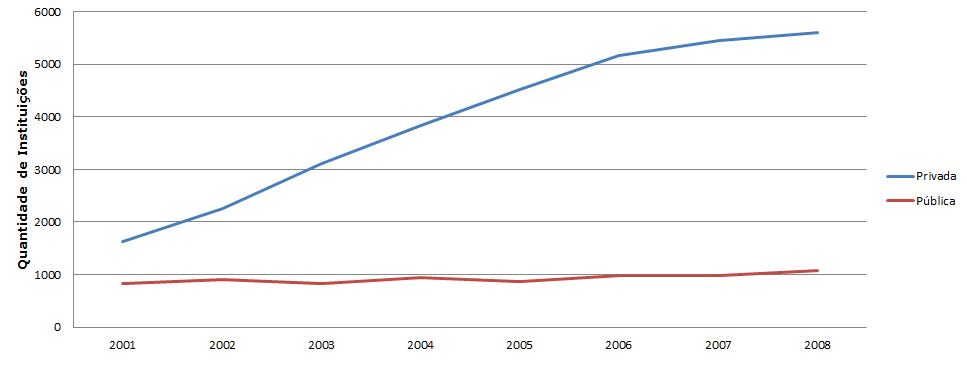
\includegraphics[width=12cm]{imagem/1.png}
	% Caption centralizada
	\captionsetup{justification=centering}
	% Caption e fonte
	\\
	\small{Fonte: Dados da Pesquisa.}
	\label{img:1}
\end{figure}

Contamos tamb�m a quantidade de Ingressantes nas institui��es (Figura \ref{img:2A}). O Resultado foi bem semelhante ao observado anteriormente. A quantidade de ingressantes aumentou consideravelmente na rede privada e se manteve constante na rede p�blica. Podemos concluir com isso que devido ao aumento do n�mero de institui��es privadas, o n�mero de ingressantes nessas institui��es tamb�m aumentou. Comparando essa conclus�o com os dados da PUC Minas (Figura \ref{img:2B}) percebe-se que o mesmo n�o ocorre nessa institui��o. O n�mero de ingressantes se mant�m praticamente inalterado durante os anos, aumentando apenas a partir de 2007. Analisando-se tamb�m os ingressos no curso de Sistemas de Informa��o (Figura \ref{img:2C}), observamos um grande aumento da procura entre os anos de 2001 e 2003. Ap�s 2003 houve uma desacelera��o na procura por esse curso, por�m seu crescimento n�o parou, apenas reduziu. Por fim, analisamos a evolu��o dos ingressantes no curso de Sistemas de Informa��o da PUC Minas (Figura \ref{img:2D}). Diferentemente do desempenho geral do curso, nessa institui��o a quantidade de ingressantes aumentou consideravelmente at� 2005, por�m apresentou uma regress�o em 2007. Ap�s esse per�odo voltou a crescer novamente.

% Figura
\begin{figure}[ht]
	\caption{\textbf{Evolu��o de Ingressantes por Rede Administrativa - MG (2001-2008)}}
	\centering
	% Arquivo da figura
	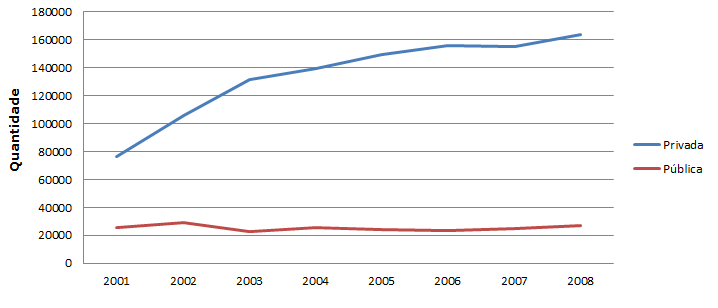
\includegraphics[width=12cm]{imagem/2A.png}
	% Caption centralizada
	\captionsetup{justification=centering}
	% Caption e fonte
	\\
	\small{Fonte: Dados da Pesquisa.}
	\label{img:2A}
\end{figure}

% Figura
\begin{figure}[ht]
	\caption{\textbf{Evolu��o de Ingressantes na PUC Minas (2001-2008)}}
	\centering
	% Arquivo da figura
	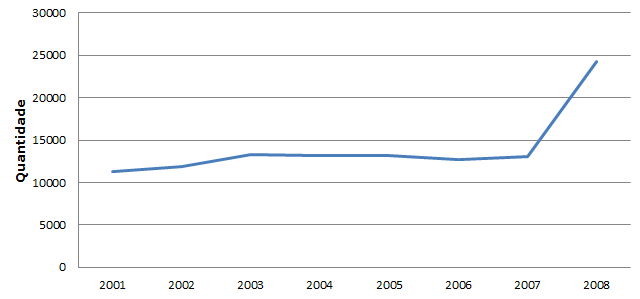
\includegraphics[width=12cm]{imagem/2B.png}
	% Caption centralizada
	\captionsetup{justification=centering}
	% Caption e fonte
	\\
	\small{Fonte: Dados da Pesquisa.}
	\label{img:2B}
\end{figure}

% Figura
\begin{figure}[ht]
	\caption{\textbf{Evolu��o de Ingressantes por Rede Administrativa nos Cursos de Sistemas de Informa��o - MG (2001-2008)}}
	\centering
	% Arquivo da figura
	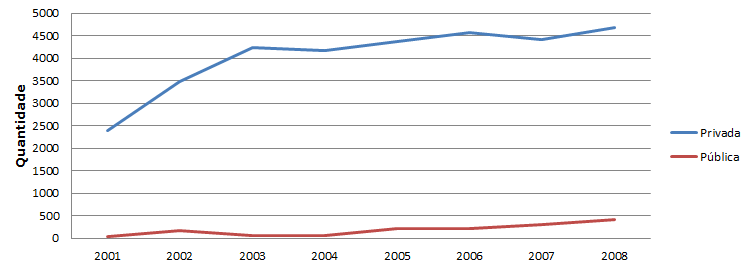
\includegraphics[width=12cm]{imagem/2C.png}
	% Caption centralizada
	\captionsetup{justification=centering}
	% Caption e fonte
	\\
	\small{Fonte: Dados da Pesquisa.}
	\label{img:2C}
\end{figure}

% Figura
\begin{figure}[ht]
	\caption{\textbf{Evolu��o de Ingressantes na PUC Minas no Curso de Sistemas de Informa��o (2001-2008)}}
	\centering
	% Arquivo da figura
	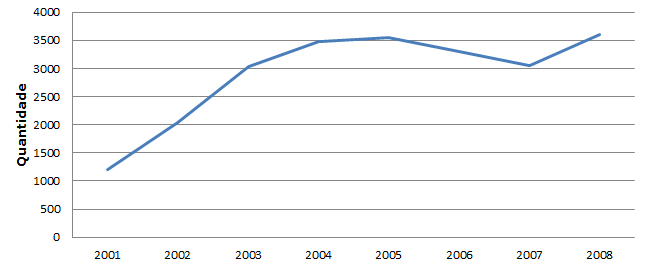
\includegraphics[width=12cm]{imagem/2D.png}
	% Caption centralizada
	\captionsetup{justification=centering}
	% Caption e fonte
	\\
	\small{Fonte: Dados da Pesquisa.}
	\label{img:2D}
\end{figure}

Afim de observar o qu�o representativo � o curso de Sistemas de Informa��o comparado aos outros, foram geradas as Figuras \ref{img:3A} e Figura \ref{img:3B}. Nelas podemos observar que dentre os cursos de todas a institui��es de Minas Gerais, Sistemas de Informa��o est� posicionado entre os top 10. Considerando apenas a PUC Minas, o curso sobe para a posi��o de quarto lugar em n�mero de ingressantes em 2008.

% Figura
\begin{figure}[ht]
	\caption{\textbf{Participa��o dos 10 maiores Cursos em rela��o ao total de Ingressantes - MG (2008)}}
	\centering
	% Arquivo da figura
	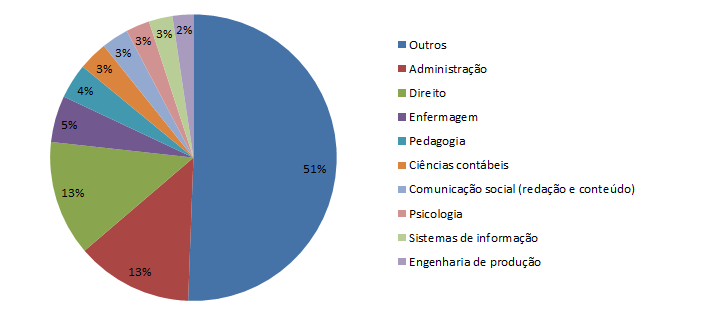
\includegraphics[width=12cm]{imagem/3A.png}
	% Caption centralizada
	\captionsetup{justification=centering}
	% Caption e fonte
	\\
	\small{Fonte: Dados da Pesquisa.}
	\label{img:3A}
\end{figure}

% Figura
\begin{figure}[ht]
	\caption{\textbf{Participa��o dos 10 maiores Cursos em rela��o ao total de Ingressantes na PUC Minas (2008)}}
	\centering
	% Arquivo da figura
	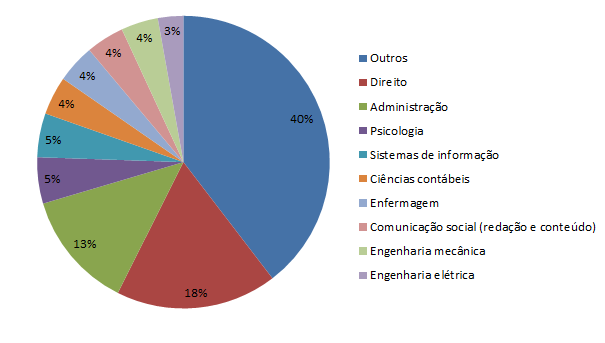
\includegraphics[width=12cm]{imagem/3B.png}
	% Caption centralizada
	\captionsetup{justification=centering}
	% Caption e fonte
	\\
	\small{Fonte: Dados da Pesquisa.}
	\label{img:3B}
\end{figure}

Afim de prever a quantidade de ingressantes para os pr�ximos 6 semestres, foi utilizado o algoritmo de previs�o do Add-in no Excel demonstrado na Figura \ref{img:4A}. Com isso verifica-se uma queda na quantidade de ingressantes, tanto para os primeiros, quanto para os segundos semestres. Nesse mesmo gr�fico aproveita-se para colocar tamb�m a representa��o da Quantidade de Evas�o. Essa se mant�m em constante crescimento. Focando esses resultados no Curso de Sistemas de Informa��o da PUC Minas Figura (\ref{img:4B}) verifica-se uma previs�o de instabilidade, com varia��o entre autos e baixos, na quantidade de ingressos e um ligeiro aumento na taxa de evas�o. 

% Figura
\begin{figure}[ht]
	\caption{\textbf{Previs�o para Ingressantes e Evas�o}}
	\centering
	% Arquivo da figura
	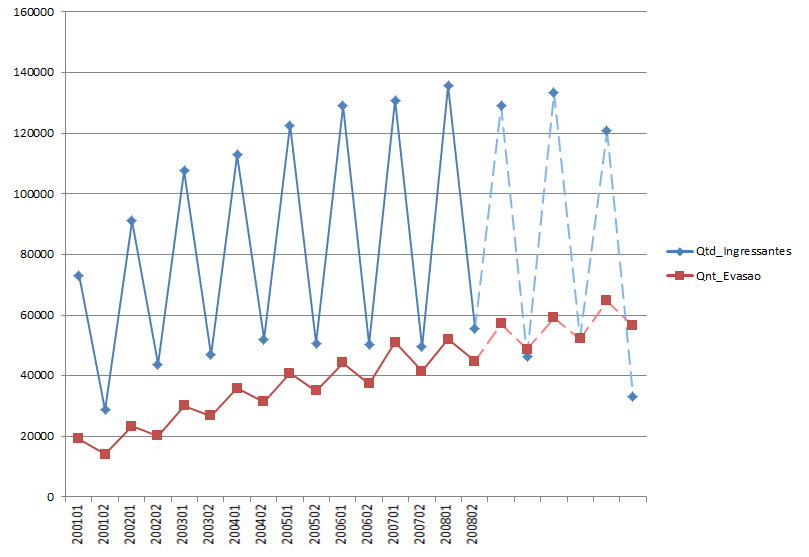
\includegraphics[width=12cm]{imagem/4A.png}
	% Caption centralizada
	\captionsetup{justification=centering}
	% Caption e fonte
	\\
	\small{Fonte: Dados da Pesquisa.}
	\label{img:4A}
\end{figure}

% Figura
\begin{figure}[ht]
	\caption{\textbf{Previs�o para Ingressantes e Evas�o no Curso de Sistemas de Informa��o da PUC Minas}}
	\centering
	% Arquivo da figura
	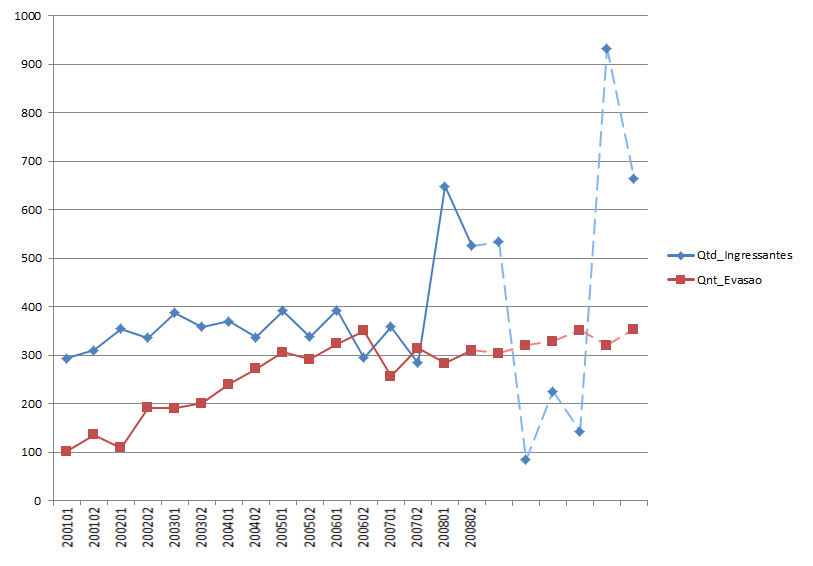
\includegraphics[width=12cm]{imagem/4B.png}
	% Caption centralizada
	\captionsetup{justification=centering}
	% Caption e fonte
	\\
	\small{Fonte: Dados da Pesquisa.}
	\label{img:4B}
\end{figure}

O pr�ximo algoritmo a ser utilizado � o de Detec��o de Categorias. Nesse Algoritmo selecionamos as colunas que possivelmente ter�o caracter�sticas em comum e ent�o � realizado o agrupamento de todos os seus elementos. Como resultado foram geradas 3 categorias:

\begin{itemize}
\item Categoria 1: Categoria com maior quantidade de elementos. Apresenta a quantidade de Candidatos/Vaga muito baixa, menor do que 1,1. A rede administrativa privada, turno noturno, �rea 	Educa��o, semestre 2 e institui��o 2098 possuem relev�ncia para que um elemento seja classificado nesse grupo.
\item Categoria 2: Nessa categoria a rela��o candidato/vaga apresenta valores entre 1 e 5. Os fatores que influenciam os itens a pertencerem a essa categoria s�o: munic�pio de Belo Horizonte, rede administrativa privada, �rea geral em Ci�ncias sociais, neg�cios e direito, curso de Direito, institui��o PUC Minas, e semestre 1.
\item Categoria 3: Para essa categoria entram os valores maiores que 5 na rela��o candidato/vaga. Tamb�m est�o inclusos como influenciadores rede administrativa p�blica, turno diurno, munic�pios de vi�osa e Ouro Preto, cursos de f�sica e hist�ria, institui��es 2047, 2058, dentre outros que podem ser visualizados na Figura \ref{img:5}.
\end{itemize}

% Figura
\begin{figure}[ht]
	\caption{\textbf{Detec��o de Categorias}}
	\centering
	% Arquivo da figura
	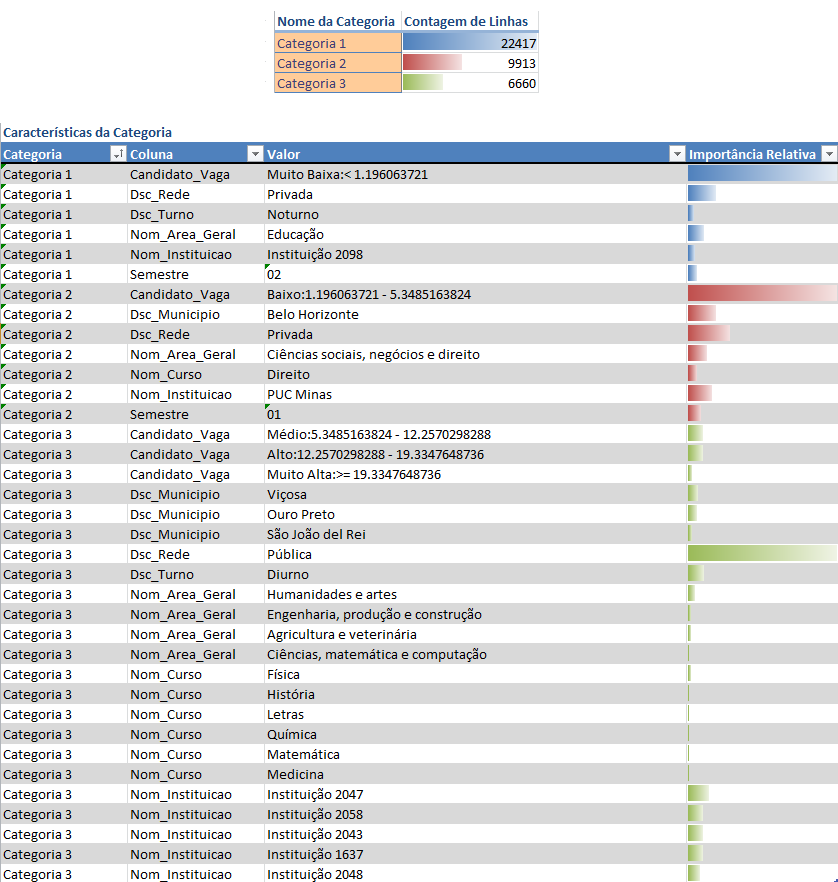
\includegraphics[width=12cm]{imagem/5.png}
	% Caption centralizada
	\captionsetup{justification=centering}
	% Caption e fonte
	\\
	\small{Fonte: Dados da Pesquisa.}
	\label{img:5}
\end{figure}

Analisando os Gr�ficos Din�micos gerados pelo Excel � poss�vel perceber que a evolu��o da quantidade de candidatos por vaga em m�dia se mant�m entre 1 e 2. Tanto para o curso de Sistemas de Informa��o da PUC Minas (Figura \ref{img:6B}), quanto para os cursos de Sistemas de Informa��o em geral(Figura \ref{img:6A}). Assim conclui-se que os padr�es gerais para os cursos de Sistema de Informa��o podem ser aplicados ao mesmo curso na PUC Minas devido ao seu estreito �ndice de correla��o.

% Figura
\begin{figure}[ht]
	\caption{\textbf{Evolu��o Candidatos/Vaga nos Cursos de Sistemas de Informa��o (2001-2008)}}
	\centering
	% Arquivo da figura
	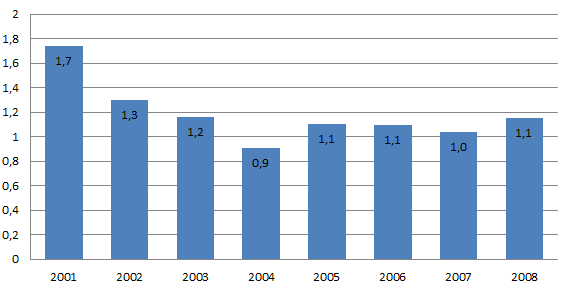
\includegraphics[width=12cm]{imagem/6A.png}
	% Caption centralizada
	\captionsetup{justification=centering}
	% Caption e fonte
	\\
	\small{Fonte: Dados da Pesquisa.}
	\label{img:6A}
\end{figure}

% Figura
\begin{figure}[ht]
	\caption{\textbf{Evolu��o Candidatos/Vaga no Curso de Sistemas de Informa��o da PUC Minas(2001-2008)}}
	\centering
	% Arquivo da figura
	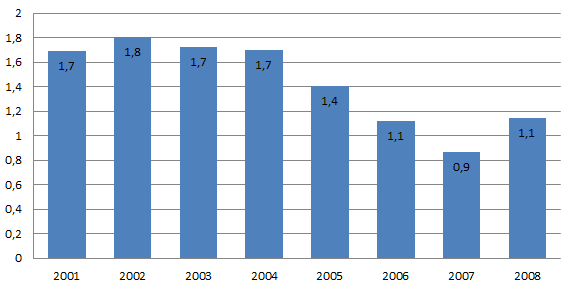
\includegraphics[width=12cm]{imagem/6B.png}
	% Caption centralizada
	\captionsetup{justification=centering}
	% Caption e fonte
	\\
	\small{Fonte: Dados da Pesquisa.}
	\label{img:6B}
\end{figure}

Usando o algoritmo An�lise de Influ�ncias sobre o Tx\_Ocupcao temos como resultado a Figura \ref{img:8}. Nessa figura s�o apresentadas as colunas que interferem no resultado do campo escolhido. Observando a barra de impacto vemos que o fato de ser o segundo semestre do ano favorece uma ocupa��o menor que 50\%. J� o fato de ser o primeiro semestre, turno noturno e IES privada favorece a ocupa��o apresentar probabilidades de 50\% a 100\%. J� a institui��o PUC Minas, o munic�pio Belo Horizonte e o curso de Direito favorecem para que a ocupa��o utrapassar seu limite.

% Figura
\begin{figure}[ht]
	\caption{\textbf{Influenciadores-chave e seu impacto sobre os valores de ``Tx\_Ocupacao''.}}
	\centering
	% Arquivo da figura
	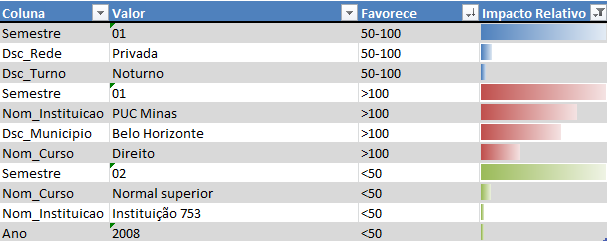
\includegraphics[width=12cm]{imagem/8.png}
	% Caption centralizada
	\captionsetup{justification=centering}
	% Caption e fonte
	\\
	\small{Fonte: Dados da Pesquisa.}
	\label{img:8}
\end{figure}

Aplicando o algoritmo An�lise da Cesta de Compras (Associa��o) obtemos rela��o de itens que acontecem em conjunto juntamente com recomenda��es. Para esse trabalho definiu-se como premissa que a taxa de ocupa��o seja maior que 50\%. Como ID foi selecionado a institui��o e como item os cursos. Para os resultados foi definido um suporte de 40\% e confian�a de 80\%. O resultado disso � apresentado pela Figura \ref{img:7A} e Figura \ref{img:7B}. Nelas observamos, por exemplo, que os cursos de Direito e Administra��o aparecem constantemente juntos quando a taxa de ocupa��o � maior que 50\% nas suas institui��es. O algor�tmo tamb�m realiza recomenda��es, ou seja, observando a Figura \ref{img:7B}, vemos que ela nos recomenda Enfermagem dado o ocorr�ncia de Fisioterapia com 91\% de precis�o. 

% Figura
\begin{figure}[ht]
	\caption{\textbf{Associa��o entre itens}}
	\centering
	% Arquivo da figura
	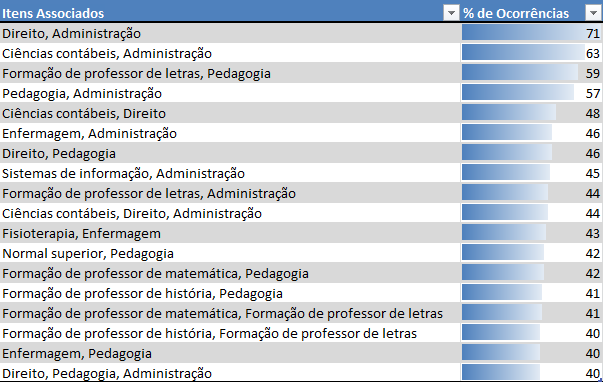
\includegraphics[width=12cm]{imagem/7A.png}
	% Caption centralizada
	\captionsetup{justification=centering}
	% Caption e fonte
	\\
	\small{Fonte: Dados da Pesquisa.}
	\label{img:7A}
\end{figure}

% Figura
\begin{figure}[ht]
	\caption{\textbf{Recomenda��es}}
	\centering
	% Arquivo da figura
	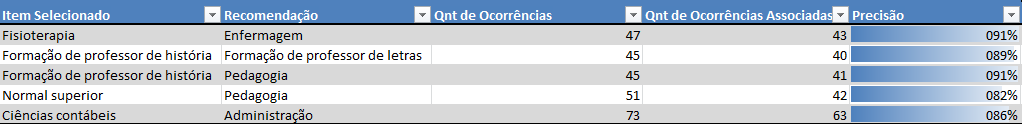
\includegraphics[width=12cm]{imagem/7B.png}
	% Caption centralizada
	\captionsetup{justification=centering}
	% Caption e fonte
	\\
	\small{Fonte: Dados da Pesquisa.}
	\label{img:7B}
\end{figure}
\capitulo{RESULTADOS E DISCUSSÕES}

\capitulo{CONCLUSÃO}

\iniciocapitulo
Discussão dos resultados obtidos na pesquisa, onde se verificam as observações pessoais do autor. Poderá também apresentar sugestões de novas linhas de estudo. A conclusão deve estar de acordo com os objetivos do trabalho. A conclusão não deve apresentar citações ou interpretações de outros autores.

\secao{Trabalhos futuros}

Criar um DW para geração dos relatorios de acordo com a dimensão escolhida.

Utilização de outros algoritimos para a resolução do problema ex. algoritimos evolutivos formiga entre outros.

%%%%%%%%%%%%%%%%%%%%%%%%%%%% P�S-TEXTUAIS %%%%%%%%%%%%%%%%%%%%%%%%%%

% Bibliografia no arquivo 'monografia.bib'
\bibliography{monografia}

%\apendice

%% Nome do Anexo
\chapter{Primeiro Ap�ndice}

% Para diminuir espa�amento entre o t�tulo e o texto
\vspace{-1.9cm}

% Texto
Textos ou documentos elaborados pelo autor, que servem como comprova��o de sua argumenta��o. Ex.: Question�rio aplicado, roteiro de entrevista, etc.


%\anexo

%% Nome do Anexo
\chapter{Primeiro Anexo}

% Para diminuir espa�amento entre o t�tulo e o texto
\vspace{-1.9cm}

% Texto
Textos ou documentos n�o elaborados pelo autor, que servem como comprova��o de sua argumenta��o. Ex.: leis na �ntegra; um folder institucional, etc.


\end{document}




